% Capitolul 6: Modele VAR și Cauzalitate Granger
% Prezentare academică de calitate Harvard
% Program de licență, Academia de Studii Economice din București

\documentclass[9pt, aspectratio=169, t]{beamer}

% Asigură încadrarea conținutului pe diapozitive
\setbeamersize{text margin left=8mm, text margin right=8mm}

%=============================================================================
% CONFIGURARE TEMĂ ȘI STIL
%=============================================================================
\usetheme{default}
% Using default theme for clean header/footer control

% Color Palette (matching Redispatch PDF)
\definecolor{MainBlue}{RGB}{26, 58, 110}
\definecolor{AccentBlue}{RGB}{26, 58, 110}
\definecolor{IDAred}{RGB}{205, 0, 0}
\definecolor{DarkGray}{RGB}{51, 51, 51}
\definecolor{MediumGray}{RGB}{128, 128, 128}
\definecolor{LightGray}{RGB}{248, 248, 248}
\definecolor{VeryLightGray}{RGB}{235, 235, 235}
\definecolor{KeynoteGray}{RGB}{218, 218, 218}
\definecolor{SectionGray}{RGB}{120, 120, 120}
\definecolor{FooterGray}{RGB}{100, 100, 100}
\definecolor{Crimson}{RGB}{220, 53, 69}
\definecolor{Forest}{RGB}{46, 125, 50}
\definecolor{Amber}{RGB}{181, 133, 63}
\definecolor{Orange}{RGB}{230, 126, 34}
\definecolor{Purple}{RGB}{142, 68, 173}

% Gradient background (exact Keynote 315° gradient: white to RGB 218,218,218)
\setbeamertemplate{background}{%
    \begin{tikzpicture}[remember picture, overlay]
        \shade[shading=axis, shading angle=315,
        top color=white, bottom color=KeynoteGray]
        (current page.south west) rectangle (current page.north east);
    \end{tikzpicture}%
}
% Fallback solid color for compatibility
\setbeamercolor{background canvas}{bg=}

\setbeamercolor{palette primary}{bg=MainBlue, fg=white}
\setbeamercolor{palette secondary}{bg=MainBlue!85, fg=white}
\setbeamercolor{palette tertiary}{bg=MainBlue!70, fg=white}
\setbeamercolor{structure}{fg=MainBlue}
\setbeamercolor{title}{fg=IDAred}
\setbeamercolor{frametitle}{fg=IDAred, bg=}
\setbeamercolor{block title}{bg=MainBlue, fg=white}
\setbeamercolor{block body}{bg=VeryLightGray, fg=DarkGray}
\setbeamercolor{block title alerted}{bg=Crimson, fg=white}
\setbeamercolor{block body alerted}{bg=Crimson!8, fg=DarkGray}
\setbeamercolor{block title example}{bg=Forest, fg=white}
\setbeamercolor{block body example}{bg=Forest!8, fg=DarkGray}
\setbeamercolor{item}{fg=MainBlue}

% Footer colors (override Madrid theme blue)
\setbeamercolor{author in head/foot}{fg=FooterGray, bg=}
\setbeamercolor{title in head/foot}{fg=FooterGray, bg=}
\setbeamercolor{date in head/foot}{fg=FooterGray, bg=}
\setbeamercolor{section in head/foot}{fg=FooterGray, bg=}
\setbeamercolor{subsection in head/foot}{fg=FooterGray, bg=}

% Bullet styles (apply everywhere including blocks)
\setbeamertemplate{itemize item}{\color{MainBlue}$\boxdot$}
\setbeamertemplate{itemize subitem}{\color{MainBlue}$\blacktriangleright$}
\setbeamertemplate{itemize subsubitem}{\color{MainBlue}\tiny$\bullet$}
\setbeamertemplate{itemize/enumerate body begin}{\normalsize}
\setbeamertemplate{itemize/enumerate subbody begin}{\normalsize}

% Item spacing - compact style
\setlength{\leftmargini}{10pt}       % Level 1: minimal indent
\setlength{\leftmarginii}{10pt}      % Level 2: minimal additional indent
% Compact list spacing (zero extra space before/after lists in blocks)
\makeatletter
\def\@listi{\leftmargin\leftmargini \topsep 0pt \parsep 0pt \itemsep 0pt}
\def\@listii{\leftmargin\leftmarginii \topsep 0pt \parsep 0pt \itemsep 0pt}
\makeatother

\setbeamertemplate{navigation symbols}{}

%=============================================================================
% CUSTOM HEADLINE
%=============================================================================
\setbeamertemplate{headline}{%
    \vskip10pt%
    \hbox to \paperwidth{%
        \hskip0.5cm%
        {\small\color{FooterGray}\renewcommand{\hyperlink}[2]{##2}\insertsectionhead}%
        \hfill%
        \textcolor{FooterGray}{\small\insertframenumber}%
        \hskip0.5cm%
    }%
    \vskip4pt%
    {\color{FooterGray}\hrule height 0.4pt}%
}

%=============================================================================
% CUSTOM FOOTER
%=============================================================================
\usepackage{fontawesome5}

\setbeamertemplate{footline}{%
    {\color{FooterGray}\hrule height 0.4pt}%
    \vskip4pt%
    \hbox to \paperwidth{%
        \hskip0.5cm%
        \textcolor{FooterGray}{\small Analiza și Prognoza Seriilor de Timp}%
        \hfill%
        \raisebox{-0.1em}{%
            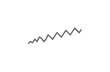
\begin{tikzpicture}[x=0.08em, y=0.08em, line width=0.4pt]
                \draw[FooterGray] (0,3) -- (1,4) -- (2,3.5) -- (3,5) -- (4,4) -- (5,6) -- (6,5.5) -- (7,4) -- (8,5) -- (9,7) -- (10,6) -- (11,5) -- (12,6.5) -- (13,8) -- (14,7) -- (15,6) -- (16,7.5) -- (17,9) -- (18,8) -- (19,7) -- (20,8.5) -- (21,10) -- (22,9) -- (23,8) -- (24,9.5);
            \end{tikzpicture}%
        }%
        \hskip0.5cm%
    }%
    \vskip6pt%
}

%=============================================================================
% PACHETE
%=============================================================================
\usepackage[utf8]{inputenc}
\usepackage[T1]{fontenc}
\usepackage{amsmath, amssymb, amsthm}
\usepackage{mathtools}
\usepackage{bm}
\usepackage{tikz}
\usetikzlibrary{arrows.meta, positioning, shapes, calc, decorations.pathreplacing, shadings}
\usepackage{booktabs}
\usepackage{multirow}
\usepackage{array}
\usepackage{graphicx}
\usepackage{hyperref}
\usepackage{colortbl}
\hypersetup{colorlinks=true, linkcolor=MainBlue, urlcolor=MainBlue}
\graphicspath{{../../logos/}{../../charts/}{../../photos/}}
\hfuzz=2pt  % Suppress tiny overfull warnings (<2pt)
\vfuzz=2pt  % Suppress tiny vertical overfull warnings (<2pt)

%=============================================================================
% COMANDA QUANTLET
%=============================================================================
\newcommand{\quantlet}[2]{%
    \hfill\href{#2}{%
        \raisebox{-0.15em}{\includegraphics[height=0.7em]{ql_logo.png}}%
        \textcolor{MainBlue}{\tiny\ #1}%
    }%
}

%=============================================================================
% MEDII PENTRU TEOREME
%=============================================================================
\theoremstyle{definition}
\setbeamertemplate{theorems}[numbered]
\newtheorem{defn}{Definiție}
\newtheorem{thm}{Teoremă}
\newtheorem{prop}{Propoziție}
\newtheorem{rmk}{Observație}

%=============================================================================
% CENTRED MINIPAGE (fără spațiu vertical suplimentar)
%=============================================================================
\newenvironment{cminipage}[1]{%
    \par\noindent\hfill\begin{minipage}{#1}\ignorespaces
}{%
    \end{minipage}\hfill\null\par
}

%=============================================================================
% COMENZI PERSONALIZATE
%=============================================================================
\newcommand{\E}{\mathbb{E}}
\newcommand{\Var}{\text{Var}}
\newcommand{\Cov}{\text{Cov}}
\newcommand{\Corr}{\text{Corr}}
\newcommand{\R}{\mathbb{R}}
\newcommand{\N}{\mathbb{N}}
\newcommand{\Z}{\mathbb{Z}}
\newcommand{\B}{\mathbf{B}}
\newcommand{\imark}{\textcolor{MainBlue}{\textbullet}}
\newcommand{\RMSE}{\text{RMSE}}
\newcommand{\MAE}{\text{MAE}}
\newcommand{\MAPE}{\text{MAPE}}
\newcommand{\bY}{\mathbf{Y}}
\newcommand{\bX}{\mathbf{X}}
\newcommand{\bA}{\mathbf{A}}
\newcommand{\bB}{\mathbf{B}}
\newcommand{\bepsilon}{\boldsymbol{\varepsilon}}
\newcommand{\bSigma}{\boldsymbol{\Sigma}}
\newcommand{\bPhi}{\boldsymbol{\Phi}}
\newcommand{\bGamma}{\boldsymbol{\Gamma}}
\newcommand{\bPi}{\boldsymbol{\Pi}}
\newcommand{\bc}{\mathbf{c}}
\newcommand{\balpha}{\boldsymbol{\alpha}}
\newcommand{\bbeta}{\boldsymbol{\beta}}

%=============================================================================
% PAGINĂ TITLU PERSONALIZATĂ
%=============================================================================
\defbeamertemplate*{title page}{hybrid}[1][]
{
    \vspace{0.2cm}
    % Logos row - top header (with clickable links)
    \begin{center}
        \href{https://www.ase.ro}{\includegraphics[height=1.0cm]{ase_logo.png}}\hspace{0.3cm}%
        \href{https://theida.net}{\includegraphics[height=1.0cm]{ida_logo.png}}\hspace{0.3cm}%
        \href{https://blockchain-research-center.com}{\includegraphics[height=1.0cm]{brc_logo.png}}\hspace{0.3cm}%
        \href{https://www.ai4efin.ase.ro}{\includegraphics[height=1.0cm]{ai4efin_logo.png}}\hspace{0.3cm}%
        \href{https://ipe.ro/new}{\includegraphics[height=1.0cm]{acad_logo.png}}\hspace{0.3cm}%
        \href{https://www.digital-finance-msca.com}{\includegraphics[height=1.0cm]{msca_logo.png}}%
    \end{center}

    \vspace{0.6cm}

    % Main title with Q logos on sides (with clickable links)
    \begin{center}
        \begin{minipage}{0.1\textwidth}
            \centering
            \href{https://quantlet.com}{\includegraphics[height=1.1cm]{ql_logo.png}}
        \end{minipage}%
        \begin{minipage}{0.78\textwidth}
            \centering
            {\LARGE\bfseries\usebeamercolor[fg]{title}\inserttitle}

            \vspace{0.3cm}

            {\usebeamerfont{subtitle}\usebeamercolor[fg]{title}\insertsubtitle}
        \end{minipage}%
        \begin{minipage}{0.1\textwidth}
            \centering
            \href{https://quantinar.com}{\includegraphics[height=1.1cm]{qr_logo.png}}
        \end{minipage}
    \end{center}

    \vspace{0.6cm}

    % Authors (left aligned)
    \hspace{0.5cm}{\usebeamerfont{author}\insertauthor}

    \vspace{0.3cm}

    % Institute/Affiliations (left aligned)
    \hspace{0.5cm}\begin{minipage}[t]{0.9\textwidth}
        \raggedright\small\insertinstitute
    \end{minipage}
}

%=============================================================================
% INFORMAȚII TITLU
%=============================================================================
\title[Analiza Seriilor de Timp]{Analiza și Prognoza Seriilor de Timp}
\subtitle{Capitolul 6: Modele VAR și Cauzalitate Granger}
\author[D.T. Pele]{Daniel Traian PELE}
\institute{Academia de Studii Economice din București\\
IDA Institute Digital Assets\\
Blockchain Research Center\\
AI4EFin Artificial Intelligence for Energy Finance\\
Academia Română, Institutul de Prognoză Economică\\
MSCA Digital Finance}
\date{}

\begin{document}

% Title page (no header/footer)
{
\setbeamertemplate{headline}{}
\setbeamertemplate{footline}{}
\begin{frame}
    \titlepage
\end{frame}
}

%=============================================================================
% OUTLINE
%=============================================================================
\begin{frame}{Cuprins}
    \vspace{-0.15cm}
    {\small
    \begin{columns}[T]
        \begin{column}{0.48\textwidth}
            \begin{block}{Fundamente}
                \begin{itemize}\setlength{\itemsep}{3pt}
                    \item Motivație
                    \item Introducere în seriile de timp multivariate
                    \item Vector Autoregresiv (VAR)
                    \item Cauzalitate Granger
                    \item Funcții de răspuns la impuls
                    \item Descompunerea varianței erorii de prognoză
                \end{itemize}
            \end{block}
        \end{column}
        \begin{column}{0.48\textwidth}
            \begin{exampleblock}{Aplicații}
                \begin{itemize}\setlength{\itemsep}{3pt}
                    \item Diagnosticarea VAR
                    \item Prognoza VAR
                    \item Exemplu practic
                    \item \mbox{Studiu de caz: PIB și Șomaj}
                    \item Rezumat și Quiz
                \end{itemize}
            \end{exampleblock}
        \end{column}
    \end{columns}
    }
\end{frame}

%=============================================================================
% LEARNING OBJECTIVES
%=============================================================================
\section{Motivație}

\begin{frame}{Obiective de învățare}
    \begin{cminipage}{0.95\textwidth}
    \begin{block}{La finalul acestui capitol, veți fi capabili să:}
        \begin{enumerate}\setlength{\itemsep}{0pt}
            \item Înțelegeți \textbf{motivația} pentru analiza multivariată a seriilor de timp
            \item Specificați și estimați modele \textbf{VAR(p)}
            \item Aplicați teste de \textbf{cauzalitate Granger}
            \item Interpretați \textbf{funcțiile de răspuns la impuls (IRF)}
            \item Efectuați \textbf{descompunerea varianței erorii de prognoză (FEVD)}
            \item Selectați ordinul optimal al lag-urilor folosind criterii informaționale
            \item Implementați analiza VAR în \textbf{Python}
        \end{enumerate}
    \end{block}
    \end{cminipage}
\end{frame}

%=============================================================================
% MOTIVATION
%=============================================================================
\begin{frame}{Exemplu motivant: Dinamica macroeconomică}
    \vspace{-0.2cm}
    \begin{columns}[T]
        \column{0.55\textwidth}
        {\scriptsize
        \begin{block}{Observații}
            \begin{itemize}\setlength{\itemsep}{0pt}
                \item Variabilele economice sunt \textbf{interconectate}: PIB afectează șomajul, inflația afectează ratele dobânzii
                \item Schimbările într-o variabilă se \textbf{propagă} prin sistem
                \item Înțelegerea acestor dinamici necesită analiză \textbf{multivariată}
            \end{itemize}
        \end{block}
        }
        \column{0.43\textwidth}
        \vspace{-0.3cm}
        \begin{center}
            \includegraphics[width=\textwidth, keepaspectratio]{ch6_motivation_econ.pdf}
        \end{center}
        \quantlet{TSA\_ch6\_motivation\_econ}{https://github.com/QuantLet/TSA/tree/main/TSA_ch6/TSA_ch6_motivation_econ}
    \end{columns}
\end{frame}

\begin{frame}{Ideea cheie: variabilele interacționează}
    \vspace{-0.2cm}
    \begin{columns}[T]
        \column{0.55\textwidth}
        {\scriptsize
        \begin{block}{Exemple}
            \begin{itemize}\setlength{\itemsep}{0pt}
                \item \textbf{Legea lui Okun}: PIB $\uparrow$ $\Rightarrow$ șomaj $\downarrow$
                \item \textbf{Regula Taylor}: Inflație $\uparrow$ $\Rightarrow$ dobândă $\uparrow$
                \item \textbf{Curba Phillips}: Compromis șomaj-inflație
            \end{itemize}
        \end{block}
        }
        \column{0.43\textwidth}
        \vspace{-0.3cm}
        \begin{center}
            \includegraphics[width=\textwidth, keepaspectratio]{ch6_motivation_scatter.pdf}
        \end{center}
        \quantlet{TSA\_ch6\_motivation\_scatter}{https://github.com/QuantLet/TSA/tree/main/TSA_ch6/TSA_ch6_motivation_scatter}
    \end{columns}
\end{frame}

\begin{frame}{Relații de avans-întârziere}
    \vspace{-0.2cm}
    \begin{columns}[T]
        \column{0.55\textwidth}
        {\scriptsize
        \begin{cminipage}{0.95\textwidth}
        \vspace{-0.2cm}
        {\footnotesize
        \begin{block}{Observații}
            \begin{itemize}\setlength{\itemsep}{0pt}
                \item Unele variabile \textbf{preced} altele: creșterea PIB prezice scăderea șomajului
                    \begin{itemize}\setlength{\itemsep}{0pt}
                        \item Corelația încrucișată relevă \textbf{sincronizarea} relațiilor
                        \item Corelație maximă la lag-ul 4: PIB-ul precede șomajul cu $\sim$4 trimestre
                    \end{itemize}
            \end{itemize}
        \end{block}
        }
        \end{cminipage}
        }
        \column{0.43\textwidth}
        \vspace{-0.3cm}
        \begin{center}
            \includegraphics[width=\textwidth, keepaspectratio]{ch6_motivation_leadlag.pdf}
        \end{center}
        \quantlet{TSA\_ch6\_motivation\_leadlag}{https://github.com/QuantLet/TSA/tree/main/TSA_ch6/TSA_ch6_motivation_leadlag}
    \end{columns}
\end{frame}

\begin{frame}{De ce modelele univariate nu sunt suficiente}
    \vspace{-0.2cm}
    \begin{columns}[T]
        \column{0.55\textwidth}
        {\scriptsize
        \begin{cminipage}{0.95\textwidth}
        \vspace{-3mm}
        {\small
        \begin{alertblock}{Problema}
            ARIMA tratează fiecare variabilă \textbf{izolat}; ignoră \textbf{interacțiunile} și \textbf{efectele de feedback}
        \end{alertblock}
        }
        \vspace{-1mm}
        {\footnotesize
        \begin{exampleblock}{Exemple}
            PIB--Șomaj, Dobândă--Inflație, Acțiuni--Volum, Curs--Balanță comercială
        \end{exampleblock}
        }
        \end{cminipage}
        }
        \column{0.43\textwidth}
        \vspace{-0.3cm}
        \begin{center}
            \includegraphics[width=\textwidth, keepaspectratio]{ch6_motivation_univariate.pdf}
        \end{center}
        \quantlet{TSA\_ch6\_motivation\_univariate}{https://github.com/QuantLet/TSA/tree/main/TSA_ch6/TSA_ch6_motivation_univariate}
    \end{columns}
\end{frame}

\begin{frame}{Ce vom învăța astăzi}
    \vspace{-0.1cm}
    \begin{cminipage}{0.95\textwidth}
    \begin{block}{Concepte fundamentale}
        {\small
        \begin{enumerate}\setlength{\itemsep}{1pt}
            \item \textbf{Modele VAR}: Cum să modelăm mai multe serii de timp împreună
            \item \textbf{Cauzalitate Granger}: Ajută $X$ la prezicerea lui $Y$?
            \item \textbf{Funcții de răspuns la impuls}: Cum se propagă șocurile?
            \item \textbf{Descompunerea varianței}: Ce determină fiecare variabilă?
        \end{enumerate}
        }
    \end{block}
    \vspace{-0.05cm}
    {\small
    \begin{exampleblock}{Exemplu recurent: Creșterea PIB și Șomajul}
        \begin{itemize}\setlength{\itemsep}{0pt}
            \item $Y_{1t}$: \textbf{Creșterea PIB} \quad și \quad $Y_{2t}$: \textbf{Rata șomajului} (\textit{Legea lui Okun})
            \item Întrebare centrală: Cauzează PIB-ul șomajul, sau invers, sau ambele?
        \end{itemize}
    \end{exampleblock}
    }
    \vspace{-0.05cm}
    {\small
    \begin{block}{Aplicații}
        \begin{itemize}\setlength{\itemsep}{0pt}
            \item Politică macroeconomică \quad\textbullet\quad Piețe financiare \quad\textbullet\quad Ciclul de afaceri \quad\textbullet\quad Managementul riscului
        \end{itemize}
    \end{block}
    }
    \end{cminipage}
\end{frame}

%=============================================================================
% SECTION 1: INTRODUCTION
%=============================================================================
\section{Introducere în seriile de timp multivariate}

\begin{frame}{Notația seriilor de timp multivariate}
    \begin{cminipage}{0.95\textwidth}
    \begin{block}{Vector de variabile}
        \begin{itemize}\setlength{\itemsep}{1pt}
            \item $\bY_t = (Y_{1t}, Y_{2t}, \ldots, Y_{Kt})'$
                \begin{itemize}\setlength{\itemsep}{0pt}
                    \item Vector $K \times 1$ de serii de timp
                \end{itemize}
            \item Exemplu cu $K=2$:
        \end{itemize}
        \vspace{-0.2cm}
        $$\bY_t = \begin{pmatrix} Y_{1t} \\ Y_{2t} \end{pmatrix} = \begin{pmatrix} \text{Creștere PIB}_t \\ \text{Șomaj}_t \end{pmatrix}$$
    \end{block}

    \vspace{0.15cm}

    \begin{block}{Întrebări cheie}
        \begin{enumerate}\setlength{\itemsep}{0pt}
            \item Ajută $Y_1$ la prezicerea lui $Y_2$? (Cauzalitate Granger)
            \item Cum afectează șocurile în $Y_1$ pe $Y_2$? (Răspunsuri la impuls)
            \item Ce proporție din varianța lui $Y_2$ se datorează lui $Y_1$? (Descompunerea varianței)
        \end{enumerate}
    \end{block}
    \end{cminipage}
\end{frame}

\begin{frame}{Staționaritate multivariată}
    \begin{cminipage}{0.95\textwidth}
    \begin{block}{Definiție: Staționaritate slabă}
        \begin{itemize}\setlength{\itemsep}{0pt}
            \item O serie de timp $K$-dimensională $\bY_t$ este \textbf{slab staționară} dacă:
                \begin{itemize}\setlength{\itemsep}{0pt}
                    \item $\E[\bY_t] = \boldsymbol{\mu}$ (vector de medie constant)
                    \item $\Cov(\bY_t, \bY_{t-h}) = \boldsymbol{\Gamma}(h)$ depinde doar de $h$, nu de $t$
                \end{itemize}
        \end{itemize}
    \end{block}

    \vspace{0.15cm}

    \begin{block}{Matricea de autocovarianță}
        \begin{itemize}\setlength{\itemsep}{0pt}
            \item \textbf{Formula}: $\boldsymbol{\Gamma}(h) = \E[(\bY_t - \boldsymbol{\mu})(\bY_{t-h} - \boldsymbol{\mu})'] = \begin{pmatrix} \gamma_{11}(h) & \gamma_{12}(h) \\ \gamma_{21}(h) & \gamma_{22}(h) \end{pmatrix}$
            \item \textbf{Proprietate}: $\boldsymbol{\Gamma}(-h) = \boldsymbol{\Gamma}(h)'$ (transpusa, nu egală!)
        \end{itemize}
    \end{block}
    \end{cminipage}
\end{frame}

\begin{frame}{Proprietăți ale covarianței încrucișate}
    \vspace{-2mm}
    \begin{cminipage}{0.95\textwidth}
    {\footnotesize
    \begin{block}{Funcția de covarianță încrucișată}
        Pentru variabilele $Y_{it}$ și $Y_{jt}$:
        $\gamma_{ij}(h) = \Cov(Y_{it}, Y_{j,t-h}) = \E[(Y_{it} - \mu_i)(Y_{j,t-h} - \mu_j)]$
    \end{block}

    \begin{alertblock}{Diferența cheie față de cazul univariat}
        \begin{itemize}\setlength{\itemsep}{0pt}
            \item În general: $\gamma_{ij}(h) \neq \gamma_{ij}(-h)$
            \item Dar: $\gamma_{ij}(h) = \gamma_{ji}(-h)$
            \item Matricea de covarianță încrucișată \textbf{nu este simetrică} pentru $h \neq 0$
        \end{itemize}
    \end{alertblock}

    \begin{exampleblock}{Exemplu}
        \begin{itemize}\setlength{\itemsep}{0pt}
            \item Dacă $Y_1$ precede $Y_2$:
                \begin{itemize}\setlength{\itemsep}{0pt}
                    \item $\gamma_{12}(h) > 0$ pentru $h > 0$
                    \item $\gamma_{12}(h) \approx 0$ pentru $h < 0$
                \end{itemize}
        \end{itemize}
    \end{exampleblock}
    }
    \end{cminipage}
\end{frame}

\begin{frame}{Matricea funcției de corelație}
    \vspace{-0.1cm}
    \begin{cminipage}{0.95\textwidth}
    \begin{block}{Definiție}
        \begin{itemize}\setlength{\itemsep}{0pt}
            \item \textbf{Matricea de autocorelație} la lag-ul $h$:
                \vspace{-0.2cm}
                $$\mathbf{R}(h) = \mathbf{D}^{-1} \boldsymbol{\Gamma}(h) \mathbf{D}^{-1}$$
                \vspace{-0.15cm}
            \item $\mathbf{D} = \text{diag}(\sigma_1, \sigma_2, \ldots, \sigma_K)$ și $\sigma_i = \sqrt{\gamma_{ii}(0)}$
        \end{itemize}
    \end{block}

    \begin{exampleblock}{Pentru cazul bivariat}
        \begin{itemize}\setlength{\itemsep}{0pt}
            \item \textbf{Matricea}: $\mathbf{R}(h) = \begin{pmatrix} \rho_{11}(h) & \rho_{12}(h) \\ \rho_{21}(h) & \rho_{22}(h) \end{pmatrix}$, unde $\rho_{ij}(h) = \frac{\gamma_{ij}(h)}{\sigma_i \sigma_j}$
            \item \textbf{Interpretare}:
                \begin{itemize}\setlength{\itemsep}{0pt}
                    \item Diagonale: ACF obișnuite
                    \item Extra-diagonale: corelații încrucișate
                \end{itemize}
        \end{itemize}
    \end{exampleblock}
    \end{cminipage}
\end{frame}

%=============================================================================
% SECTION 2: VAR MODELS
%=============================================================================
\section{Vector Autoregresiv (VAR)}

\begin{frame}{Portret de cercetător: Sims \& Granger}
    \vspace{-0.2cm}
    \begin{columns}[T]
        \begin{column}{0.22\textwidth}
            \centering
            \includegraphics[width=0.95\textwidth, height=0.22\textheight, keepaspectratio]{photo_christopher_sims.jpg}
            \\[0.05cm]
            {\tiny\textcolor{MediumGray}{Christopher Sims (*1942)}}\\[-0.05cm]
            {\tiny\textcolor{MediumGray}{Premiul Nobel 2011}}\\[0.02cm]
            \href{https://en.wikipedia.org/wiki/Christopher_A._Sims}{\faWikipediaW\ \textcolor{MainBlue}{\tiny Wikipedia (en)}}
        \end{column}
        \begin{column}{0.76\textwidth}
            \begin{block}{Biografie}
                {\footnotesize \begin{itemize}\setlength{\itemsep}{0pt}
                    \item \textbf{Christopher Sims}: econometrist american la Princeton. Premiul Nobel (2011) ,,pentru cercetări empirice privind cauza și efectul în macroeconomie''
                    \item \textbf{Clive Granger}: economist britanic-american la UC San Diego. Premiul Nobel (2003) ,,pentru metode de analiză a seriilor economice cu tendințe comune (cointegrare)''
                \end{itemize}}
            \end{block}
        \end{column}
    \end{columns}
    \vspace{0.1cm}
    \begin{columns}[T]
        \begin{column}{0.22\textwidth}
            \centering
            \includegraphics[width=0.95\textwidth, height=0.22\textheight, keepaspectratio]{photo_clive_granger.jpg}
            \\[0.05cm]
            {\tiny\textcolor{MediumGray}{Clive Granger (1934--2009)}}\\[-0.05cm]
            {\tiny\textcolor{MediumGray}{Premiul Nobel 2003}}\\[0.02cm]
            \href{https://en.wikipedia.org/wiki/Clive_Granger}{\faWikipediaW\ \textcolor{MainBlue}{\tiny Wikipedia (en)}}
        \end{column}
        \begin{column}{0.76\textwidth}
            \begin{exampleblock}{Contribuții principale}
                {\footnotesize
                \begin{itemize}\setlength{\itemsep}{0pt}
                    \item \textbf{Modele VAR} (Sims, 1980) --- vectori autoregresivi pentru macroeconomie
                    \item \textbf{Cauzalitatea Granger} (Granger, 1969) --- concept de cauzalitate predictivă
                    \item \textbf{Funcții impuls-răspuns} și identificarea VAR structural
                    \item \textbf{Cointegrarea} (Granger, 1981) --- relații de echilibru pe termen lung
                \end{itemize}}
            \end{exampleblock}
        \end{column}
    \end{columns}
\end{frame}

\begin{frame}{Modelul VAR(p)}
    \begin{cminipage}{0.95\textwidth}
    \begin{block}{Definiție}
        \begin{itemize}\setlength{\itemsep}{0pt}
            \item Un model \textbf{VAR(p)} pentru $K$ variabile:
                $$\bY_t = \mathbf{c} + \bA_1 \bY_{t-1} + \bA_2 \bY_{t-2} + \cdots + \bA_p \bY_{t-p} + \bepsilon_t$$
                \vspace{-0.15cm}
            \item $\bY_t$: vector $K \times 1$ de variabile endogene
            \item $\mathbf{c}$: vector $K \times 1$ de constante
            \item $\bA_i$: matrice de coeficienți $K \times K$
            \item $\bepsilon_t$: vector $K \times 1$ de termeni de eroare cu $\E[\bepsilon_t] = \mathbf{0}$, $\E[\bepsilon_t \bepsilon_t'] = \bSigma$
        \end{itemize}
    \end{block}
    \end{cminipage}
\end{frame}

\begin{frame}{VAR(1) cu două variabile}
    \begin{cminipage}{0.95\textwidth}
    \begin{block}{VAR(1) bivariat}
        \begin{itemize}\setlength{\itemsep}{0pt}
            \item Forma matriceală:
                $$\begin{pmatrix} Y_{1t} \\ Y_{2t} \end{pmatrix} = \begin{pmatrix} c_1 \\ c_2 \end{pmatrix} + \begin{pmatrix} a_{11} & a_{12} \\ a_{21} & a_{22} \end{pmatrix} \begin{pmatrix} Y_{1,t-1} \\ Y_{2,t-1} \end{pmatrix} + \begin{pmatrix} \varepsilon_{1t} \\ \varepsilon_{2t} \end{pmatrix}$$
        \end{itemize}
    \end{block}

    \vspace{0.15cm}

    \begin{exampleblock}{Ecuație cu ecuație}
        \begin{itemize}\setlength{\itemsep}{0pt}
            \item \textbf{Ecuația 1}: $Y_{1t} = c_1 + a_{11} Y_{1,t-1} + a_{12} Y_{2,t-1} + \varepsilon_{1t}$
            \item \textbf{Ecuația 2}: $Y_{2t} = c_2 + a_{21} Y_{1,t-1} + a_{22} Y_{2,t-1} + \varepsilon_{2t}$
            \item \textbf{Ideea cheie}: Fiecare ecuație include lag-uri ale \textbf{tuturor} variabilelor!
        \end{itemize}
    \end{exampleblock}
    \end{cminipage}
\end{frame}

\begin{frame}{Exemplu numeric: VAR(1)}
    \vspace{-2mm}
    \begin{cminipage}{0.95\textwidth}
    {\footnotesize
    \begin{exampleblock}{Model VAR(1) specific}
        Exemplu numeric:
        $$\begin{pmatrix} Y_{1t} \\ Y_{2t} \end{pmatrix} = \begin{pmatrix} 0.5 \\ 0.3 \end{pmatrix} + \begin{pmatrix} 0.7 & 0.2 \\ -0.1 & 0.6 \end{pmatrix} \begin{pmatrix} Y_{1,t-1} \\ Y_{2,t-1} \end{pmatrix} + \begin{pmatrix} \varepsilon_{1t} \\ \varepsilon_{2t} \end{pmatrix}$$
        \vspace{-2mm}
    \end{exampleblock}

    \begin{block}{Interpretarea coeficienților}
        \begin{itemize}\setlength{\itemsep}{0pt}
            \item $a_{11} = 0.7$: Creștere de 1 în $Y_1$ la $t\!-\!1$ $\Rightarrow$ $Y_1$ la $t$ crește cu 0.7
            \item $a_{12} = 0.2$: Creștere de 1 în $Y_2$ la $t\!-\!1$ $\Rightarrow$ $Y_1$ la $t$ crește cu 0.2
            \item $a_{21} = -0.1$: Creștere de 1 în $Y_1$ la $t\!-\!1$ $\Rightarrow$ $Y_2$ la $t$ \textbf{scade} cu 0.1
            \item $a_{22} = 0.6$: Creștere de 1 în $Y_2$ la $t\!-\!1$ $\Rightarrow$ $Y_2$ la $t$ crește cu 0.6
        \end{itemize}
    \end{block}
    }
    \end{cminipage}
\end{frame}

\begin{frame}{VAR(2): dinamică de ordin superior}
    \vspace{-0.15cm}
    \begin{cminipage}{0.95\textwidth}
    {\small
    \begin{block}{Specificația VAR(2)}
        \begin{itemize}\setlength{\itemsep}{0pt}
            \item Forma generală: $\bY_t = \mathbf{c} + \bA_1 \bY_{t-1} + \bA_2 \bY_{t-2} + \bepsilon_t$
            \item Pentru $K=2$, $p=2$: fiecare ecuație are $1 + pK = 5$ parametri, total $K(1 + pK) = 10$
        \end{itemize}
    \end{block}
    }

    \vspace{-0.1cm}

    {\small
    \begin{exampleblock}{Dezvoltat}
        \begin{itemize}\setlength{\itemsep}{0pt}
            \item Ecuațiile individuale:
                \vspace{-0.2cm}
                \begin{align*}
                    Y_{1t} &= c_1 + a_{11}^{(1)} Y_{1,t-1} + a_{12}^{(1)} Y_{2,t-1} + a_{11}^{(2)} Y_{1,t-2} + a_{12}^{(2)} Y_{2,t-2} + \varepsilon_{1t} \\
                    Y_{2t} &= c_2 + a_{21}^{(1)} Y_{1,t-1} + a_{22}^{(1)} Y_{2,t-1} + a_{21}^{(2)} Y_{1,t-2} + a_{22}^{(2)} Y_{2,t-2} + \varepsilon_{2t}
                \end{align*}
                \vspace{-0.15cm}
        \end{itemize}
    \end{exampleblock}
    }

    \vspace{-0.1cm}
    {\scriptsize
    \begin{alertblock}{Blestemul dimensionalității}
        \begin{itemize}\setlength{\itemsep}{0pt}
            \item VAR($p$) cu $K$ variabile are $K + pK^2$ parametri; cu $K=5$, $p=4$: $5 + 4 \times 25 = 105$ parametri!
        \end{itemize}
    \end{alertblock}
    }
    \end{cminipage}
\end{frame}

\begin{frame}{Proces VAR simulat}
    \vspace{-0.2cm}
    \begin{columns}[T]
        \column{0.55\textwidth}
        {\scriptsize
        \begin{block}{Observații}
            \begin{itemize}\setlength{\itemsep}{1pt}
                \item Proces VAR(1) bivariat simulat --- interdependența dintre serii
                \item Fiecare variabilă răspunde la propriul trecut și trecutul celeilalte variabile
                \item Dinamica încrucișată vizibilă
            \end{itemize}
        \end{block}
        }
        \column{0.43\textwidth}
        \vspace{-0.3cm}
        \begin{center}
            \includegraphics[width=\textwidth, keepaspectratio]{ch6_var_simulation.pdf}
        \end{center}
        \hfill\quantlet{TSA\_ch6\_var\_simulation}{https://github.com/QuantLet/TSA/tree/main/TSA_ch6/TSA_ch6_var_simulation}
    \end{columns}
\end{frame}

\begin{frame}{Forma companion}
    \vspace{-3mm}
    \begin{cminipage}{0.95\textwidth}
    {\small
    \begin{block}{Conversia VAR(p) la VAR(1)}
        Orice VAR($p$) poate fi scris ca VAR(1) în \textbf{forma companion}: $\boldsymbol{\xi}_t = \mathbf{A} \boldsymbol{\xi}_{t-1} + \mathbf{v}_t$
    \end{block}
    }
    \vspace{-1mm}
    {\footnotesize
    \begin{exampleblock}{Pentru VAR(2)}
        \textbf{Forma}: $\underbrace{\begin{pmatrix} \bY_t \\ \bY_{t-1} \end{pmatrix}}_{\boldsymbol{\xi}_t} = \underbrace{\begin{pmatrix} \bA_1 & \bA_2 \\ \mathbf{I}_K & \mathbf{0} \end{pmatrix}}_{\mathbf{A}} \underbrace{\begin{pmatrix} \bY_{t-1} \\ \bY_{t-2} \end{pmatrix}}_{\boldsymbol{\xi}_{t-1}} + \underbrace{\begin{pmatrix} \bepsilon_t \\ \mathbf{0} \end{pmatrix}}_{\mathbf{v}_t}$
        \quad \textbf{Dimensiune}: $\mathbf{A}$ este $Kp \times Kp$
    \end{exampleblock}
    }
    \vspace{-1mm}
    {\scriptsize
    \begin{alertblock}{Produsul Kronecker $\otimes$}
        Dacă $\mathbf{A}$ este $m \times n$ și $\mathbf{B}$ este $p \times q$, atunci $\mathbf{A} \otimes \mathbf{B}$ este matricea $mp \times nq$:
        \vspace{-2mm}
        $$\mathbf{A} \otimes \mathbf{B} = \begin{pmatrix} a_{11}\mathbf{B} & \cdots & a_{1n}\mathbf{B} \\ \vdots & \ddots & \vdots \\ a_{m1}\mathbf{B} & \cdots & a_{mn}\mathbf{B} \end{pmatrix}$$
        \vspace{-4mm}

        \textbf{Utilizare}: $\text{vec}(\boldsymbol{\Sigma}_Y) = (\mathbf{I}_{K^2} - \mathbf{A} \otimes \mathbf{A})^{-1}\, \text{vec}(\boldsymbol{\Sigma}_\varepsilon)$ --- matricea de covarianță a VAR staționar.
    \end{alertblock}
    }
    \end{cminipage}
\end{frame}

\begin{frame}{Staționaritatea VAR}
    \begin{cminipage}{0.95\textwidth}
    \begin{block}{Condiția de stabilitate}
        \begin{itemize}\setlength{\itemsep}{0pt}
            \item VAR(p) este \textbf{stabil} (staționar) dacă toate rădăcinile lui:
                $$\det(\mathbf{I}_K - \bA_1 z - \bA_2 z^2 - \cdots - \bA_p z^p) = 0$$
                \vspace{-0.15cm}
            \item Se află \textbf{în afara} cercului unitate (adică $|z| > 1$)
        \end{itemize}
    \end{block}

    \vspace{0.15cm}

    \begin{alertblock}{Pentru VAR(1)}
        \begin{itemize}\setlength{\itemsep}{2pt}
            \item Modelul este stabil dacă toate \textbf{valorile proprii} ale lui $\bA_1$ sunt mai mici decât 1 în valoare absolută
            \item Exemplu: Pentru $\bA_1 = \begin{pmatrix} 0.5 & 0.1 \\ 0.2 & 0.3 \end{pmatrix}$, valorile proprii sunt $\lambda_1 \approx 0.54$ și $\lambda_2 \approx 0.26$
                \begin{itemize}\setlength{\itemsep}{0pt}
                    \item Ambele $< 1$ $\succ$ stabil!
                \end{itemize}
        \end{itemize}
    \end{alertblock}
    \end{cminipage}
\end{frame}

\begin{frame}{Condiția de stabilitate: interpretare vizuală}
    \vspace{-0.2cm}
    {\scriptsize
    \begin{block}{Observații}
        \begin{itemize}\setlength{\itemsep}{0pt}
            \item Valorile proprii ale matricei companion trebuie să fie în interiorul cercului unitate (cele complexe vin în perechi conjugate)
            \item VAR exploziv (nestaționar) dacă vreo valoare proprie este în afara cercului
        \end{itemize}
    \end{block}
    }
    \begin{center}
        \includegraphics[width=0.95\textwidth, height=0.50\textheight, keepaspectratio]{ch6_stability_roots.pdf}
    \end{center}
    \quantlet{TSA\_ch6\_stability\_roots}{https://github.com/QuantLet/TSA/tree/main/TSA_ch6/TSA_ch6_stability_roots}
\end{frame}

\begin{frame}{Calculul valorilor proprii: exemplu}
    \vspace{-2mm}
    \begin{cminipage}{0.95\textwidth}
    {\footnotesize
    \begin{block}{Pentru $\bA = \begin{pmatrix} 0.7 & 0.2 \\ -0.1 & 0.6 \end{pmatrix}$}
        Polinomul caracteristic: $\det(\bA - \lambda \mathbf{I}) = 0$
        $$\det\begin{pmatrix} 0.7 - \lambda & 0.2 \\ -0.1 & 0.6 - \lambda \end{pmatrix} = (0.7-\lambda)(0.6-\lambda) + 0.02 = 0$$
        \vspace{-0.2cm}
        $$\lambda^2 - 1.3\lambda + 0.44 = 0$$
        \vspace{-0.2cm}
    \end{block}

    \begin{exampleblock}{Soluție}
        Folosind formula de gradul 2:
        $$\lambda = \frac{1.3 \pm \sqrt{1.69 - 1.76}}{2} = \frac{1.3 \pm \sqrt{-0.07}}{2} = 0.65 \pm 0.132i$$
        \vspace{-0.2cm}
        $|\lambda| = \sqrt{0.65^2 + 0.132^2} = \sqrt{0.44} = 0.663 < 1$ \quad $\checkmark$ Stabil!
    \end{exampleblock}
    }
    \end{cminipage}
\end{frame}

\begin{frame}{Media unui VAR staționar}
    \begin{cminipage}{0.95\textwidth}
    \begin{block}{Media necondiționată}
        \begin{itemize}\setlength{\itemsep}{2pt}
            \item Pentru un VAR(1) staționar: $\bY_t = \mathbf{c} + \bA \bY_{t-1} + \bepsilon_t$
            \item Luând medii: $\E[\bY_t] = \mathbf{c} + \bA \E[\bY_{t-1}]$
            \item Deoarece $\E[\bY_t] = \E[\bY_{t-1}] = \boldsymbol{\mu}$ (staționaritate):
                $$\boldsymbol{\mu} = \mathbf{c} + \bA \boldsymbol{\mu} \quad \succ \quad \boldsymbol{\mu} = (\mathbf{I}_K - \bA)^{-1} \mathbf{c}$$
                \vspace{-0.15cm}
        \end{itemize}
    \end{block}

    {\small
    \begin{exampleblock}{Exemplu}
        Dacă $\mathbf{c} = \begin{pmatrix} 0.5 \\ 0.3 \end{pmatrix}$ și $\bA = \begin{pmatrix} 0.7 & 0.2 \\ -0.1 & 0.6 \end{pmatrix}$:
        \vspace{-0.2cm}
        $$\boldsymbol{\mu} = \begin{pmatrix} 0.3 & -0.2 \\ 0.1 & 0.4 \end{pmatrix}^{-1} \begin{pmatrix} 0.5 \\ 0.3 \end{pmatrix} = \frac{1}{0.14}\begin{pmatrix} 0.4 & 0.2 \\ -0.1 & 0.3 \end{pmatrix}\begin{pmatrix} 0.5 \\ 0.3 \end{pmatrix} = \begin{pmatrix} 1.86 \\ 0.29 \end{pmatrix}$$
        \vspace{-0.2cm}
    \end{exampleblock}
    }
    \end{cminipage}
\end{frame}

\begin{frame}{Structura covarianței pentru VAR(1)}
    \vspace{-2mm}
    \begin{cminipage}{0.95\textwidth}
    {\footnotesize
    \begin{block}{Matricea varianță-covarianță $\boldsymbol{\Gamma}(0)$}
        Pentru VAR(1), varianța satisface \textbf{ecuația discretă Lyapunov}:
        $\boldsymbol{\Gamma}(0) = \bA \boldsymbol{\Gamma}(0) \bA' + \bSigma$
    \end{block}

    \begin{block}{Autocovarianța la lag-ul $h$}
        Formula: $\boldsymbol{\Gamma}(h) = \bA^h \boldsymbol{\Gamma}(0), \quad h \geq 0$.
        Autocovarianțele scad geometric cu valorile proprii ale lui $\bA$.
    \end{block}

    \begin{alertblock}{Rezolvarea ecuației Lyapunov}
        Se rezolvă prin vectorizare:
        $\text{vec}(\boldsymbol{\Gamma}(0)) = (\mathbf{I}_{K^2} - \bA \otimes \bA)^{-1} \text{vec}(\bSigma)$,
        unde $\otimes$ denotă produsul Kronecker.
    \end{alertblock}
    }
    \end{cminipage}
\end{frame}

\begin{frame}{Estimarea VAR}
    \vspace{-0.1cm}
    \begin{cminipage}{0.95\textwidth}
    \begin{block}{Estimarea OLS}
        \begin{itemize}\setlength{\itemsep}{0pt}
            \item Fiecare ecuație poate fi estimată prin \textbf{OLS separat}:
                \vspace{-0.15cm}
                $$\hat{\bA} = \left(\sum_{t=1}^{T} \bY_{t-1} \bY_{t-1}'\right)^{-1} \left(\sum_{t=1}^{T} \bY_{t-1} \bY_t'\right)$$
                \vspace{-0.2cm}
            \item Eficientă deoarece toate ecuațiile au \textbf{aceiași regresori}
        \end{itemize}
    \end{block}

    \begin{block}{Matricea de covarianță}
        Estimatorul: $\hat{\bSigma} = \frac{1}{T-Kp-1} \sum_{t=1}^{T} \hat{\bepsilon}_t \hat{\bepsilon}_t'$

        Erorile $\varepsilon_{1t}$ și $\varepsilon_{2t}$ pot fi \textbf{corelate contemporan}.
    \end{block}
    \end{cminipage}
\end{frame}

\begin{frame}{Selecția lag-ului: exemplu}
    \vspace{-0.2cm}
    \begin{columns}[T]
        \column{0.55\textwidth}
        {\scriptsize
        \begin{block}{Observații}
            \begin{itemize}\setlength{\itemsep}{0pt}
                \item Date reale SUA (FRED): PIB și Șomaj, $T = 140$ trimestre
                \item Criterii informaționale: AIC și BIC pentru lag $p = 1, \ldots, 10$ (pot sugera ordine diferite)
                \item Interpretare: valori mici = ajustare mai bună; ambele selectează $p = 2$
            \end{itemize}
        \end{block}
        }
        \column{0.43\textwidth}
        \vspace{-0.3cm}
        \begin{center}
            \includegraphics[width=\textwidth, keepaspectratio]{ch6_lag_selection.pdf}
        \end{center}
        \quantlet{TSA\_ch6\_lag\_selection}{https://github.com/QuantLet/TSA/tree/main/TSA_ch6/TSA_ch6_lag_selection}
    \end{columns}
\end{frame}

\begin{frame}{Selecția ordinului lag-ului}
    \vspace{-2mm}
    \begin{cminipage}{0.95\textwidth}
    {\small
    \begin{block}{Criterii informaționale}
        Alegem $p$ care minimizează:
        \vspace{-0.2cm}
        \begin{align*}
            \text{AIC}(p) &= \ln|\hat{\bSigma}_p| + \frac{2pK^2}{T} \\[-0.05cm]
            \text{BIC}(p) &= \ln|\hat{\bSigma}_p| + \frac{pK^2 \ln T}{T} \\[-0.05cm]
            \text{HQ}(p) &= \ln|\hat{\bSigma}_p| + \frac{2pK^2 \ln\ln T}{T}
        \end{align*}
        \vspace{-0.2cm}
        {\scriptsize \textbf{unde:} $\hat{\bSigma}_p$ = matricea de covarianță a reziduurilor, $K$ = nr.\ variabile, $p$ = nr.\ lag-uri, $T$ = dimensiunea eșantionului}
    \end{block}
    }

    {\small
    \begin{block}{Îndrumări}
        \begin{itemize}\setlength{\itemsep}{0pt}
            \item Comportamentul criteriilor:
                \begin{itemize}\setlength{\itemsep}{0pt}
                    \item AIC tinde să selecteze modele \textbf{mai mari} (mai bune pentru prognoză)
                    \item BIC tinde să selecteze modele \textbf{mai mici} (selecție consistentă)
                \end{itemize}
            \item Începeți cu $p_{max}$ bazat pe frecvența datelor (ex. 4 pentru trimestrial, 12 pentru lunar)
        \end{itemize}
    \end{block}
    }
    \end{cminipage}
\end{frame}

\begin{frame}{Modele VAR restricționate}
    \vspace{-0.3cm}
    \begin{cminipage}{0.95\textwidth}
    {\footnotesize
    \begin{block}{De ce restricționăm?}
        \begin{itemize}\setlength{\itemsep}{0pt}
            \item Modelele VAR complete pot fi \textbf{supraparametrizate}:
                \begin{itemize}\setlength{\itemsep}{0pt}
                    \item Mulți coeficienți pot fi nesemnificativi
                    \item Prognoze slabe
                    \item Pierdere de grade de libertate
                \end{itemize}
        \end{itemize}
    \end{block}

    \begin{block}{Restricții comune}
        \begin{itemize}\setlength{\itemsep}{0pt}
            \item \textbf{Restricții de zero}: Setăm coeficienți mici la zero
            \item \textbf{Exogenitate de bloc}: Unele variabile nu afectează altele
            \item \textbf{Excluderea lag-urilor}: Excludem anumite lag-uri
        \end{itemize}
    \end{block}

    \begin{alertblock}{Testarea restricțiilor}
        \begin{itemize}\setlength{\itemsep}{0pt}
            \item Folosim testul raportului de verosimilitate:
            \item $LR = T(\ln|\hat{\bSigma}_R| - \ln|\hat{\bSigma}_U|) \sim \chi^2_r$, unde $r$ = numărul de restricții
        \end{itemize}
    \end{alertblock}
    }
    \end{cminipage}
\end{frame}

%=============================================================================
% SECTION 3: GRANGER CAUSALITY
%=============================================================================
\section{Cauzalitate Granger}

\begin{frame}{Ce este cauzalitatea Granger?}
    \begin{cminipage}{0.95\textwidth}
    \begin{block}{Clive Granger (1969, Premiul Nobel 2003)}
        \begin{itemize}\setlength{\itemsep}{0pt}
            \item ``$X$ \textbf{cauzează Granger} pe $Y$'' dacă valorile trecute ale lui $X$ ajută la prezicerea lui $Y$, \textbf{dincolo de} ce pot prezice valorile trecute ale lui $Y$ singure
        \end{itemize}
    \end{block}

    \vspace{0.15cm}

    \begin{alertblock}{Distincție importantă: Cauzalitate Granger $\neq$ Cauzalitate reală}
        \begin{itemize}\setlength{\itemsep}{0pt}
            \item Cauzalitatea Granger este despre \textbf{conținut predictiv}
            \item NU implică cauzare economică/structurală
            \item ``$X$ cauzează Granger pe $Y$'' înseamnă: $X$ conține informații utile pentru prognoza lui $Y$
        \end{itemize}
    \end{alertblock}
    \end{cminipage}
\end{frame}

\begin{frame}{Definiție formală}
    \begin{cminipage}{0.95\textwidth}
    \begin{block}{Cauzalitate Granger}
        \begin{itemize}\setlength{\itemsep}{1pt}
            \item $X$ \textbf{nu cauzează Granger} pe $Y$ dacă:
        \end{itemize}
        \vspace{-0.2cm}
        $$\E[Y_t | Y_{t-1}, Y_{t-2}, \ldots, X_{t-1}, X_{t-2}, \ldots] = \E[Y_t | Y_{t-1}, Y_{t-2}, \ldots]$$
        \vspace{-0.15cm}
        \begin{itemize}\setlength{\itemsep}{0pt}
            \item Adăugarea istoricului lui $X$ nu îmbunătățește predicția lui $Y$
        \end{itemize}
    \end{block}

    \vspace{0.1cm}

    \begin{exampleblock}{În contextul VAR}
        \begin{itemize}\setlength{\itemsep}{1pt}
            \item VAR(1): $Y_{1t} = c_1 + a_{11} Y_{1,t-1} + a_{12} Y_{2,t-1} + \varepsilon_{1t}$
                \begin{itemize}\setlength{\itemsep}{0pt}
                    \item $Y_2$ \textbf{nu} cauzează Granger pe $Y_1$ dacă $a_{12} = 0$
                \end{itemize}
            \item VAR(p): nu cauzează dacă $a_{12}^{(1)} = a_{12}^{(2)} = \cdots = a_{12}^{(p)} = 0$
        \end{itemize}
    \end{exampleblock}
    \end{cminipage}
\end{frame}

\begin{frame}{Testarea cauzalității Granger}
    \vspace{-0.1cm}
    \begin{cminipage}{0.95\textwidth}
    \begin{block}{Ipotezele testului}
        \begin{itemize}\setlength{\itemsep}{1pt}
            \item $H_0$: $Y_2$ \textbf{nu} cauzează Granger pe $Y_1$
                \begin{itemize}\setlength{\itemsep}{0pt}
                    \item $a_{12}^{(1)} = a_{12}^{(2)} = \cdots = a_{12}^{(p)} = 0$
                \end{itemize}
            \item $H_1$: Cel puțin un $a_{12}^{(i)} \neq 0$
                \begin{itemize}\setlength{\itemsep}{0pt}
                    \item Există cauzalitate Granger
                \end{itemize}
        \end{itemize}
    \end{block}

    \begin{block}{Statistica testului: Testul Wald}
        \begin{itemize}\setlength{\itemsep}{0pt}
            \item \textbf{Formula}: $F = \frac{(RSS_R - RSS_U)/p}{RSS_U/(T-2p-1)} \sim F_{p, T-2p-1}$
            \item $RSS_R$: Reziduuri model restricționat (fără lag-urile lui $Y_2$)
            \item $RSS_U$: Reziduuri model nerestricționat (VAR complet)
        \end{itemize}
    \end{block}
    \end{cminipage}
\end{frame}

\begin{frame}{Tipuri de cauzalitate Granger}
    \vspace{-2mm}
    \begin{cminipage}{0.95\textwidth}
    \begin{center}
    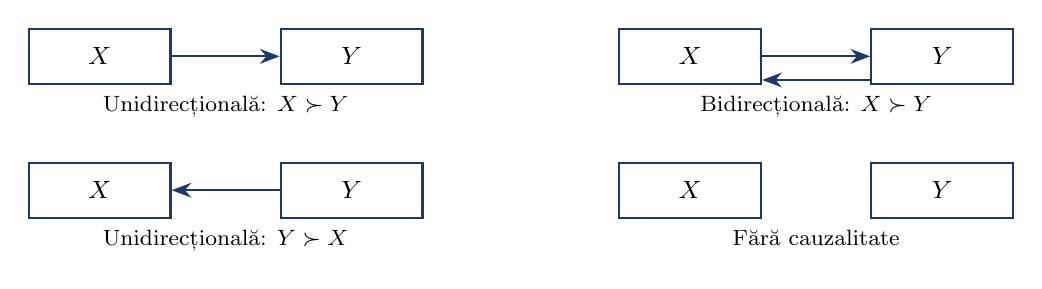
\begin{tikzpicture}[
        box/.style={rectangle, draw=MainBlue, thick, minimum width=1.8cm, minimum height=0.7cm, font=\small},
        arrow/.style={-{Stealth[length=2.5mm]}, thick, MainBlue}
    ]
        % Unidirectional X -> Y
        \node[box] (x1) at (0, 1.7) {$X$};
        \node[box] (y1) at (3.2, 1.7) {$Y$};
        \draw[arrow] (x1) -- (y1);
        \node[below=0.02cm of x1, xshift=1.6cm, font=\footnotesize] {Unidirecțională: $X \succ Y$};

        % Unidirectional Y -> X
        \node[box] (x2) at (0, 0) {$X$};
        \node[box] (y2) at (3.2, 0) {$Y$};
        \draw[arrow] (y2) -- (x2);
        \node[below=0.02cm of x2, xshift=1.6cm, font=\footnotesize] {Unidirecțională: $Y \succ X$};

        % Bidirectional
        \node[box] (x3) at (7.5, 1.7) {$X$};
        \node[box] (y3) at (10.7, 1.7) {$Y$};
        \draw[arrow] (x3.east) -- (y3.west);
        \draw[arrow] (y3.west) ++(0, -0.3) -- (x3.east |- {0, 1.4});
        \node[below=0.02cm of x3, xshift=1.6cm, font=\footnotesize] {Bidirecțională: $X \succ Y$};

        % No causality
        \node[box] (x4) at (7.5, 0) {$X$};
        \node[box] (y4) at (10.7, 0) {$Y$};
        \node[below=0.02cm of x4, xshift=1.6cm, font=\footnotesize] {Fără cauzalitate};
    \end{tikzpicture}
    \end{center}
    \vspace{1mm}
    {\small
    \begin{block}{Exemple economice}
        \begin{itemize}\setlength{\itemsep}{0pt}
            \item Masa monetară $\succ$ Producție? (viziunea monetaristă)
            \item Prețurile acțiunilor $\succ$ Volumul tranzacționat (bidirecțională)
            \item Vremea $\succ$ Recolta (unidirecțională, evident)
        \end{itemize}
    \end{block}
    }
    \end{cminipage}
\end{frame}

\begin{frame}{Corelație încrucișată: ilustrare vizuală}
    \vspace{-0.2cm}
    {\scriptsize
    \begin{block}{Interpretare}
        \begin{itemize}\setlength{\itemsep}{0pt}
            \item Stânga: două serii înrudite; Dreapta: CCF relevă că $X$ precede $Y$ (corelații semnificative la lag-uri pozitive)
        \end{itemize}
    \end{block}
    }
    \begin{center}
        \includegraphics[width=0.95\textwidth, height=0.50\textheight, keepaspectratio]{ch6_def_ccf.pdf}
    \end{center}
    \quantlet{TSA\_ch6\_def\_ccf}{https://github.com/QuantLet/TSA/tree/main/TSA_ch6/TSA_ch6_def_ccf}
\end{frame}

\begin{frame}{Funcția de corelație încrucișată}
    \vspace{-0.1cm}
    \begin{cminipage}{0.95\textwidth}
    {\small
    \begin{defn}[Funcția de corelație încrucișată]
        \begin{itemize}\setlength{\itemsep}{0pt}
            \item \textbf{Corelația încrucișată} între $X_t$ și $Y_t$ la lag-ul $k$:
        \end{itemize}
        \vspace{-0.2cm}
        $$\rho_{XY}(k) = \frac{\gamma_{XY}(k)}{\sigma_X \sigma_Y} = \frac{\Cov(X_t, Y_{t+k})}{\sqrt{\Var(X_t)\Var(Y_t)}}$$
        \vspace{-0.15cm}
    \end{defn}

    \begin{block}{Interpretare}
        \begin{itemize}\setlength{\itemsep}{0pt}
            \item $\rho_{XY}(k) > 0$ la $k > 0$: $X$ este corelat pozitiv cu $Y$ viitor (X poate precede Y)
            \item $\rho_{XY}(k) > 0$ la $k < 0$: $X$ este corelat pozitiv cu $Y$ trecut (Y poate precede X)
        \end{itemize}
    \end{block}

    \begin{alertblock}{Notă}
        \begin{itemize}\setlength{\itemsep}{0pt}
            \item Spre deosebire de ACF, corelația încrucișată \textbf{nu este simetrică}: $\rho_{XY}(k) \neq \rho_{XY}(-k)$ în general
        \end{itemize}
    \end{alertblock}
    }
    \end{cminipage}
\end{frame}

\begin{frame}{Cauzalitate Granger: considerații practice}
    \begin{cminipage}{0.95\textwidth}
    \begin{alertblock}{Capcane comune}
        \begin{enumerate}\setlength{\itemsep}{0pt}
            \item \textbf{Variabile omise}: O a treia variabilă $Z$ poate cauza atât $X$ cât și $Y$
            \item \textbf{Nestaționaritate}: Testul necesită date staționare (sau cointegrare)
            \item \textbf{Selecția lag-ului}: Rezultatele pot fi sensibile la $p$
            \item \textbf{Mărimea eșantionului}: Necesită suficiente observații
        \end{enumerate}
    \end{alertblock}

    {\small
    \begin{block}{Bune practici}
        \begin{itemize}\setlength{\itemsep}{0pt}
            \item Pregătirea datelor: testați pentru rădăcini unitare; folosiți criterii multiple pentru selecția lag-ului
            \item Robustețe: verificați la diferite ordine ale lag-ului; raportați rezultatele pentru ambele direcții
        \end{itemize}
    \end{block}
    }
    \end{cminipage}
\end{frame}

\begin{frame}{Test cauzalitate Granger: exemplu numeric}
    \begin{cminipage}{0.95\textwidth}
    {\small
    \begin{exampleblock}{Testare: Cauzează creșterea masei monetare Granger producția?}
        \begin{itemize}\setlength{\itemsep}{1pt}
            \item \textbf{Model nerestricționat} (VAR cu 2 lag-uri):
        \end{itemize}
        \vspace{-0.2cm}
        $$\Delta Y_t = c + \alpha_1 \Delta Y_{t-1} + \alpha_2 \Delta Y_{t-2} + \beta_1 \Delta M_{t-1} + \beta_2 \Delta M_{t-2} + \varepsilon_t$$
        \vspace{-0.15cm}
        \begin{itemize}\setlength{\itemsep}{1pt}
            \item \textbf{Model restricționat} ($H_0$: $\beta_1 = \beta_2 = 0$):
        \end{itemize}
        \vspace{-0.2cm}
        $$\Delta Y_t = c + \alpha_1 \Delta Y_{t-1} + \alpha_2 \Delta Y_{t-2} + \varepsilon_t$$
    \end{exampleblock}

    \begin{block}{Calculul testului}
        $T = 100$, $RSS_U = 45.2$, $RSS_R = 52.8$:
        \vspace{-0.2cm}
        $$F = \frac{(52.8 - 45.2)/2}{45.2/(100 - 5)} = \frac{3.8}{0.476} = 7.98$$
        \vspace{-0.2cm}
        $F_{0.05}(2, 95) = 3.09$ $\succ$ \textbf{Respingem $H_0$}: Banii cauzează Granger producția!
    \end{block}
    }
    \end{cminipage}
\end{frame}

\begin{frame}{Procedura Toda-Yamamoto}
    \vspace{-0.2cm}
    \begin{cminipage}{0.95\textwidth}
    {\footnotesize
    \begin{alertblock}{Problema cu datele nestaționare}
        \begin{itemize}\setlength{\itemsep}{0pt}
            \item Testul Granger standard are \textbf{distribuții non-standard} când:
                \begin{itemize}\setlength{\itemsep}{0pt}
                    \item Variabilele au rădăcini unitare
                    \item Variabilele sunt cointegrate
                \end{itemize}
        \end{itemize}
    \end{alertblock}

    \begin{block}{Soluția Toda-Yamamoto (1995)}
        \begin{enumerate}\setlength{\itemsep}{0pt}
            \item Determinăm ordinul maxim de integrare $d_{max}$
            \item Estimăm VAR($p + d_{max}$) în \textbf{niveluri}
            \item Testăm restricții doar pe primele $p$ lag-uri
            \item Lag-urile suplimentare $d_{max}$ \textbf{nu sunt} testate (doar pentru distribuția corectă)
        \end{enumerate}
    \end{block}

    \begin{exampleblock}{Avantaj}
        \begin{itemize}\setlength{\itemsep}{0pt}
            \item Testul Wald are distribuție asimptotică $\chi^2$ indiferent de cointegrare!
        \end{itemize}
    \end{exampleblock}
    }
    \end{cminipage}
\end{frame}

\begin{frame}{Cauzalitate instantanee}
    \vspace{-0.25cm}
    \begin{cminipage}{0.95\textwidth}
    {\scriptsize
    \begin{block}{Definiție}
        \begin{itemize}\setlength{\itemsep}{1pt}
            \item $X$ \textbf{cauzează instantaneu} pe $Y$ dacă:
                \begin{itemize}\setlength{\itemsep}{0pt}
                    \item $\E[Y_t | \Omega_{t-1}, X_t] \neq \E[Y_t | \Omega_{t-1}]$
                    \item $\Omega_{t-1}$: toate informațiile trecute
                \end{itemize}
        \end{itemize}
    \end{block}

    \begin{block}{Testarea în VAR}
        Testăm $\sigma_{12} \neq 0$ în $\bSigma = \begin{pmatrix} \sigma_1^2 & \sigma_{12} \\ \sigma_{12} & \sigma_2^2 \end{pmatrix}$. \quad $\sigma_{12} = 0$ $\succ$ fără cauzalitate instantanee.
    \end{block}

    \begin{alertblock}{Interpretare}
        Cauze posibile: \textbf{șocuri comune} sau \textbf{agregarea datelor} --- nu neapărat efecte contemporane reale.
    \end{alertblock}
    }
    \end{cminipage}
\end{frame}

\begin{frame}{Cauzalitate Granger în sisteme multiple}
    \begin{cminipage}{0.95\textwidth}
    \begin{block}{Testul exogenității de bloc}
        \begin{itemize}\setlength{\itemsep}{0pt}
            \item Într-un VAR cu $K > 2$ variabile, testăm dacă un \textbf{grup} de variabile cauzează Granger un alt grup
            \item Exemplu: Cauzează variabilele financiare (rate ale dobânzii, prețuri acțiuni) Granger variabilele reale (PIB, șomaj)?
        \end{itemize}
    \end{block}

    \begin{exampleblock}{Statistica testului}
        $\chi^2 = T \left(\ln|\hat{\bSigma}_R| - \ln|\hat{\bSigma}_U|\right) \sim \chi^2_{K_1 \cdot K_2 \cdot p}$,
        unde $K_1$ = variabile ``cauzate'', $K_2$ = variabile ``cauzatoare''.
    \end{exampleblock}
    \end{cminipage}
\end{frame}

%=============================================================================
% SECTION 4: IMPULSE RESPONSE FUNCTIONS
%=============================================================================
\section{Funcții de răspuns la impuls}

\begin{frame}{Ce sunt funcțiile de răspuns la impuls?}
    \vspace{-0.2cm}
    \begin{cminipage}{0.95\textwidth}
    {\small
    \begin{block}{Definiție}
        \begin{itemize}\setlength{\itemsep}{1pt}
            \item \textbf{Funcție de Răspuns la Impuls (IRF)}
                \begin{itemize}\setlength{\itemsep}{0pt}
                    \item Efectul unui șoc punctual la o variabilă
                    \item Asupra valorilor curente și viitoare ale tuturor variabilelor
                \end{itemize}
        \end{itemize}
    \end{block}

    \begin{exampleblock}{Întrebarea la care răspund IRF-urile}
        \begin{itemize}\setlength{\itemsep}{0pt}
            \item ``Dacă apare un șoc de 1 unitate la $Y_1$ astăzi, ce se întâmplă cu $Y_1$ și $Y_2$ în următoarele $h$ perioade?''
        \end{itemize}
    \end{exampleblock}

    \begin{block}{Reprezentarea MA($\infty$)}
        Un VAR(p) stabil: $\bY_t = \boldsymbol{\mu} + \sum_{i=0}^{\infty} \boldsymbol{\Phi}_i \bepsilon_{t-i}$,
        unde $\boldsymbol{\Phi}_i$ = \textbf{răspunsurile la impuls} la orizontul $i$.
    \end{block}
    }
    \end{cminipage}
\end{frame}

\begin{frame}{Calculul IRF pentru VAR(1)}
    \begin{cminipage}{0.95\textwidth}
    \begin{block}{Pentru VAR(1): $\bY_t = \mathbf{c} + \bA \bY_{t-1} + \bepsilon_t$}
        \begin{itemize}\setlength{\itemsep}{0pt}
            \item Matricele de răspuns la impuls sunt:
                $$\boldsymbol{\Phi}_0 = \mathbf{I}_K, \quad \boldsymbol{\Phi}_1 = \bA, \quad \boldsymbol{\Phi}_2 = \bA^2, \quad \ldots, \quad \boldsymbol{\Phi}_h = \bA^h$$
                \vspace{-0.15cm}
        \end{itemize}
    \end{block}

    \vspace{0.15cm}

    \begin{exampleblock}{Interpretare}
        \begin{itemize}\setlength{\itemsep}{1pt}
            \item $[\boldsymbol{\Phi}_h]_{ij}$: Efectul asupra lui $Y_i$ la $t+h$
                \begin{itemize}\setlength{\itemsep}{0pt}
                    \item Al unui șoc unitar la $Y_j$ la momentul $t$
                \end{itemize}
            \item VAR stabil: $\boldsymbol{\Phi}_h \succ \mathbf{0}$ când $h \succ \infty$
                \begin{itemize}\setlength{\itemsep}{0pt}
                    \item Șocurile dispar în timp
                \end{itemize}
        \end{itemize}
    \end{exampleblock}
    \end{cminipage}
\end{frame}

\begin{frame}{Calculul IRF pentru VAR(p) general}
    \vspace{-0.1cm}
    \begin{cminipage}{0.95\textwidth}
    {\small
    \begin{block}{Formula recursivă pentru VAR(p)}
        \begin{itemize}\setlength{\itemsep}{0pt}
            \item Pentru $\bY_t = \mathbf{c} + \bA_1\bY_{t-1} + \cdots + \bA_p\bY_{t-p} + \bepsilon_t$:
                $$\boldsymbol{\Phi}_h = \sum_{j=1}^{\min(h,p)} \bA_j \boldsymbol{\Phi}_{h-j}, \quad h = 1, 2, 3, \ldots$$
                \vspace{-0.15cm}
            \item Cu $\boldsymbol{\Phi}_0 = \mathbf{I}_K$ și $\boldsymbol{\Phi}_h = \mathbf{0}$ pentru $h < 0$
        \end{itemize}
    \end{block}

    \begin{exampleblock}{Exemplu: IRF pentru VAR(2)}
        \begin{itemize}\setlength{\itemsep}{0pt}
            \item $\boldsymbol{\Phi}_0 = \mathbf{I}_K$
            \item $\boldsymbol{\Phi}_1 = \bA_1 \boldsymbol{\Phi}_0 = \bA_1$
            \item $\boldsymbol{\Phi}_2 = \bA_1 \boldsymbol{\Phi}_1 + \bA_2 \boldsymbol{\Phi}_0 = \bA_1^2 + \bA_2$
            \item $\boldsymbol{\Phi}_3 = \bA_1 \boldsymbol{\Phi}_2 + \bA_2 \boldsymbol{\Phi}_1 = \bA_1(\bA_1^2 + \bA_2) + \bA_2\bA_1$
        \end{itemize}
    \end{exampleblock}
    }
    \end{cminipage}
\end{frame}

\begin{frame}{Funcții de răspuns la impuls: exemplu}
    \vspace{-0.2cm}
    \begin{columns}[T]
        \column{0.55\textwidth}
        {\scriptsize
        \begin{block}{Observații}
            \begin{itemize}\setlength{\itemsep}{2pt}
                \item Răspunsul fiecărei variabile la un șoc unitar
                \item Zonele umbrite = intervale de încredere
                \item VAR stabil: răspunsurile converg la zero
            \end{itemize}
        \end{block}
        }
        \column{0.43\textwidth}
        \vspace{-0.3cm}
        \begin{center}
            \includegraphics[width=\textwidth, keepaspectratio]{ch6_irf.pdf}
        \end{center}
        \hfill\quantlet{TSA\_ch6\_irf}{https://github.com/QuantLet/TSA/tree/main/TSA_ch6/TSA_ch6_irf}
    \end{columns}
\end{frame}

\begin{frame}{IRF ortogonalizate}
    \vspace{-0.15cm}
    \begin{cminipage}{0.95\textwidth}
    {\small
    \begin{alertblock}{Problema: Erori corelate}
        \begin{itemize}\setlength{\itemsep}{0pt}
            \item $\bSigma$ nu este diagonală
                \begin{itemize}\setlength{\itemsep}{0pt}
                    \item Șocurile $\varepsilon_{1t}$ și $\varepsilon_{2t}$ sunt corelate
                    \item Un șoc la ``$Y_1$'' implică și un șoc la ``$Y_2$''
                \end{itemize}
        \end{itemize}
    \end{alertblock}

    \begin{block}{Soluție: Descompunerea Cholesky}
        \begin{itemize}\setlength{\itemsep}{0pt}
            \item Factorizare: $\bSigma = \mathbf{P}\mathbf{P}'$ ($\mathbf{P}$: inferior triunghiulară)
            \item Șocuri ortogonalizate: $\mathbf{u}_t = \mathbf{P}^{-1}\bepsilon_t$ cu $\E[\mathbf{u}_t \mathbf{u}_t'] = \mathbf{I}$
            \item IRF ortogonalizate: $\boldsymbol{\Theta}_h = \boldsymbol{\Phi}_h \mathbf{P}$
        \end{itemize}
    \end{block}

    \begin{alertblock}{Ordinea contează!}
        \begin{itemize}\setlength{\itemsep}{0pt}
            \item De la ``cea mai exogenă'' la ``cea mai endogenă''
                \begin{itemize}\setlength{\itemsep}{0pt}
                    \item Rezultatele depind de ordinea variabilelor
                \end{itemize}
        \end{itemize}
    \end{alertblock}
    }
    \end{cminipage}
\end{frame}

\begin{frame}{Exemplu numeric IRF}
    \vspace{-3mm}
    \begin{cminipage}{0.95\textwidth}
    {\footnotesize
    \begin{block}{Pentru $\bA = \begin{pmatrix} 0.7 & 0.2 \\ -0.1 & 0.6 \end{pmatrix}$}
        Calculul matricelor IRF:
        \vspace{-2mm}
                \begin{align*}
                    \boldsymbol{\Phi}_0 &= \begin{pmatrix} 1 & 0 \\ 0 & 1 \end{pmatrix}, \quad
                    \boldsymbol{\Phi}_1 = \bA = \begin{pmatrix} 0.7 & 0.2 \\ -0.1 & 0.6 \end{pmatrix}, \quad
                    \boldsymbol{\Phi}_2 = \bA^2 = \begin{pmatrix} 0.47 & 0.26 \\ -0.13 & 0.34 \end{pmatrix}
                \end{align*}
        \vspace{-4mm}
    \end{block}

    \begin{exampleblock}{Interpretare}
        \begin{itemize}\setlength{\itemsep}{0pt}
            \item $[\boldsymbol{\Phi}_2]_{12} = 0.26$: Un șoc unitar la $Y_2$ crește $Y_1$ cu 0.26 după 2 perioade
            \item $[\boldsymbol{\Phi}_2]_{21} = -0.13$: Un șoc unitar la $Y_1$ \textbf{scade} $Y_2$ cu 0.13 după 2 perioade
        \end{itemize}
    \end{exampleblock}
    }
    \end{cminipage}
\end{frame}

\begin{frame}{Răspunsuri la impuls cumulative}
    \begin{cminipage}{0.95\textwidth}
    \begin{block}{Definiție}
        \begin{itemize}\setlength{\itemsep}{0pt}
            \item \textbf{IRF cumulativ} până la orizontul $H$:
                $\boldsymbol{\Psi}_H = \sum_{h=0}^{H} \boldsymbol{\Phi}_h$
            \item Măsoară \textbf{efectul total acumulat} al unui șoc
        \end{itemize}
    \end{block}

    \vspace{0.1cm}

    \begin{exampleblock}{Multiplicatorul pe termen lung}
        \begin{itemize}\setlength{\itemsep}{0pt}
            \item Pentru VAR stabil: $\boldsymbol{\Psi}_\infty = (\mathbf{I}_K - \bA_1 - \bA_2 - \cdots - \bA_p)^{-1}$
            \item Aceasta dă \textbf{efectul permanent} al unui șoc punctual
        \end{itemize}
    \end{exampleblock}

    \vspace{0.1cm}

    {\footnotesize
    \begin{alertblock}{Când să folosim}
        \begin{itemize}\setlength{\itemsep}{0pt}
            \item IRF cumulative sunt utile când ne interesează impactul total (ex.\ pierderea cumulată de PIB după un șoc)
        \end{itemize}
    \end{alertblock}
    }
    \end{cminipage}
\end{frame}

\begin{frame}{Intervale de încredere pentru IRF}
    \vspace{-0.2cm}
    \begin{cminipage}{0.95\textwidth}
    {\footnotesize
    \begin{block}{Surse de incertitudine}
        \begin{itemize}\setlength{\itemsep}{0pt}
            \item IRF sunt funcții de parametrii estimați $\hat{\bA}_1, \ldots, \hat{\bA}_p$, deci au \textbf{incertitudine de eșantionare}
        \end{itemize}
    \end{block}

    \begin{block}{Metode pentru benzi de încredere}
        \begin{enumerate}\setlength{\itemsep}{0pt}
            \item \textbf{Asimptotice}: Folosim metoda delta pentru a deriva erorile standard
            \item \textbf{Monte Carlo}: Simulăm din distribuția asimptotică a lui $\hat{\bA}$
            \item \textbf{Bootstrap}: Reeșantionăm reziduurile și reestimăm VAR
        \end{enumerate}
    \end{block}

    \begin{alertblock}{Procedura Bootstrap}
        \begin{enumerate}\setlength{\itemsep}{0pt}
            \item Estimăm VAR, salvăm reziduurile $\{\hat{\bepsilon}_t\}$
            \item Extragem cu înlocuire pentru a crea $\{\hat{\bepsilon}_t^*\}$
            \item Generăm eșantion bootstrap folosind VAR estimat
            \item Reestimăm și calculăm IRF
            \item Repetăm de $B$ ori; folosim percentilele pentru IC
        \end{enumerate}
    \end{alertblock}
    }
    \end{cminipage}
\end{frame}

\begin{frame}{VAR structural (SVAR)}
    \begin{cminipage}{0.95\textwidth}
    \begin{block}{Motivație}
        \begin{itemize}\setlength{\itemsep}{0pt}
            \item Șocurile VAR standard $\bepsilon_t$ sunt inovații de \textbf{formă redusă} $\succ$ combinații liniare de șocuri structurale
            \item Vrem să identificăm \textbf{șocuri structurale} semnificative economic
        \end{itemize}
    \end{block}

    \vspace{0.15cm}

    \begin{block}{Forma structurală}
        \begin{itemize}\setlength{\itemsep}{0pt}
            \item Modelul structural:
                $$\mathbf{B}_0 \bY_t = \boldsymbol{\Gamma}_0 + \mathbf{B}_1 \bY_{t-1} + \cdots + \mathbf{B}_p \bY_{t-p} + \mathbf{u}_t$$
                \vspace{-0.15cm}
            \item $\mathbf{u}_t$ sunt \textbf{șocuri structurale} cu $\E[\mathbf{u}_t \mathbf{u}_t'] = \mathbf{I}_K$
        \end{itemize}
    \end{block}

    \vspace{0.15cm}

    {\footnotesize
    \begin{exampleblock}{Relația cu forma redusă}
        \begin{itemize}\setlength{\itemsep}{0pt}
            \item $\bepsilon_t = \mathbf{B}_0^{-1} \mathbf{u}_t \quad \succ \quad \bSigma = \mathbf{B}_0^{-1} (\mathbf{B}_0^{-1})'$
        \end{itemize}
    \end{exampleblock}
    }
    \end{cminipage}
\end{frame}

\begin{frame}{Exemplu IRF structural}
    \vspace{-0.2cm}
    {\scriptsize
    \begin{block}{Observații}
        \begin{itemize}\setlength{\itemsep}{0pt}
            \item IRF structurale (Cholesky) --- ordinea variabilelor afectează interpretarea
            \item Restricții contemporane: prima variabilă reacționează doar la propriile șocuri
        \end{itemize}
    \end{block}
    }
    \begin{center}
        \includegraphics[width=0.95\textwidth, height=0.50\textheight, keepaspectratio]{ch6_structural_irf.pdf}
    \end{center}
    \quantlet{TSA\_ch6\_structural\_irf}{https://github.com/QuantLet/TSA/tree/main/TSA_ch6/TSA_ch6_structural_irf}
\end{frame}

\begin{frame}{Identificare în SVAR}
    \vspace{-0.2cm}
    \begin{cminipage}{0.95\textwidth}
    {\small
    \begin{alertblock}{Problema identificării}
        \begin{itemize}\setlength{\itemsep}{0pt}
            \item $\bSigma$ are $K(K+1)/2$ elemente unice, dar $\mathbf{B}_0^{-1}$ are $K^2$ elemente
            \item Avem nevoie de $K(K-1)/2$ restricții suplimentare!
        \end{itemize}
    \end{alertblock}

    \begin{block}{Scheme comune de identificare}
        \begin{enumerate}\setlength{\itemsep}{0pt}
            \item \textbf{Restricții pe termen scurt}: Efecte de impact zero (Cholesky)
            \item \textbf{Restricții pe termen lung}: Efecte zero pe termen lung (Blanchard-Quah)
            \item \textbf{Restricții de semn}: Constrângeri de inegalitate pe IRF
            \item \textbf{Instrumente externe}: Folosim informații din afară
        \end{enumerate}
    \end{block}

    \begin{exampleblock}{Exemplu: Ordonare Cholesky (recursivă)}
        \begin{itemize}\setlength{\itemsep}{0pt}
            \item Pentru $K=2$: $\mathbf{B}_0^{-1} = \begin{pmatrix} b_{11} & 0 \\ b_{21} & b_{22} \end{pmatrix}$
            \item Variabila 1 nu răspunde la șocul 2 contemporan
        \end{itemize}
    \end{exampleblock}
    }
    \end{cminipage}
\end{frame}

%=============================================================================
% SECTION 5: FORECAST ERROR VARIANCE DECOMPOSITION
%=============================================================================
\section{Descompunerea varianței erorii de prognoză}

\begin{frame}{FEVD: Exemplu}
    \vspace{-0.2cm}
    {\scriptsize
    \begin{block}{Observații}
        \begin{itemize}\setlength{\itemsep}{0pt}
            \item Proporția varianței prognozei atribuibilă fiecărui șoc structural
            \item Dinamica temporală: orizonturi scurte --- șocuri proprii domină; efectele încrucișate cresc în timp
        \end{itemize}
    \end{block}
    }
    \begin{center}
        \includegraphics[width=0.95\textwidth, height=0.50\textheight, keepaspectratio]{ch6_fevd.pdf}
    \end{center}
    \quantlet{TSA\_ch6\_fevd}{https://github.com/QuantLet/TSA/tree/main/TSA_ch6/TSA_ch6_fevd}
\end{frame}

\begin{frame}{Descompunerea varianței}
    \begin{cminipage}{0.95\textwidth}
    \begin{alertblock}{Întrebare}
        \begin{itemize}\setlength{\itemsep}{0pt}
            \item Ce proporție din varianța erorii de prognoză a lui $Y_i$ la orizontul $h$ se datorează șocurilor la $Y_j$?
        \end{itemize}
    \end{alertblock}

    \begin{block}{Formula FEVD}
        \vspace{-0.2cm}
        $$\text{FEVD}_{ij}(h) = \frac{\sum_{s=0}^{h-1} [\boldsymbol{\Theta}_s]_{ij}^2}{\sum_{s=0}^{h-1} \sum_{k=1}^{K} [\boldsymbol{\Theta}_s]_{ik}^2}$$
        \vspace{-0.2cm}
        \begin{itemize}\setlength{\itemsep}{0pt}
            \item Dă \textbf{procentul} din varianța prognozei la $h$ pași a lui $Y_i$ explicat de șocurile la $Y_j$
        \end{itemize}
    \end{block}

    {\small
    \begin{exampleblock}{Proprietăți}
        \begin{itemize}\setlength{\itemsep}{0pt}
            \item $0 \leq \text{FEVD}_{ij}(h) \leq 1$
            \item $\sum_{j=1}^{K} \text{FEVD}_{ij}(h) = 1$ (suma la 100\%)
            \item La $h=1$: Șocurile proprii domină (prin construcția Cholesky)
        \end{itemize}
    \end{exampleblock}
    }
    \end{cminipage}
\end{frame}

\begin{frame}{FEVD: Exemplu numeric}
    \vspace{-0.15cm}
    \begin{cminipage}{0.95\textwidth}
    {\footnotesize
    \begin{block}{Calculul FEVD pentru VAR bivariat}
        \begin{itemize}\setlength{\itemsep}{0pt}
            \item Folosind IRF ortogonalizate $\boldsymbol{\Theta}_h$, FEVD la orizontul $H$:
                $$\text{FEVD}_{11}(H) = \frac{\sum_{h=0}^{H-1} \theta_{11}^2(h)}{\sum_{h=0}^{H-1} [\theta_{11}^2(h) + \theta_{12}^2(h)]}$$
                \vspace{-0.15cm}
        \end{itemize}
    \end{block}

    \begin{exampleblock}{Exemplu de calcul}
        \begin{center}
        \begin{tabular}{c|cc|cc}
            \toprule
            $h$ & $\theta_{11}(h)$ & $\theta_{12}(h)$ & $\theta_{11}^2(h)$ & $\theta_{12}^2(h)$ \\
            \midrule
            0 & 1.00 & 0.00 & 1.00 & 0.00 \\
            1 & 0.70 & 0.20 & 0.49 & 0.04 \\
            2 & 0.47 & 0.26 & 0.22 & 0.07 \\
            \bottomrule
        \end{tabular}
        \end{center}
        \begin{itemize}\setlength{\itemsep}{0pt}
            \item $\text{FEVD}_{11}(3) = \frac{1.00 + 0.49 + 0.22}{1.00 + 0.49 + 0.22 + 0.00 + 0.04 + 0.07} = \frac{1.71}{1.82} = 94\%$
        \end{itemize}
    \end{exampleblock}
    }
    \end{cminipage}
\end{frame}

\begin{frame}{Descompunerea istorică: Exemplu}
    \vspace{-0.2cm}
    {\scriptsize
    \begin{block}{Observații}
        \begin{itemize}\setlength{\itemsep}{0pt}
            \item Contribuții structurale: fiecare culoare = un șoc diferit, stivuite însumează abaterea de la medie
            \item Utilitate: identifică șocurile din episoadele istorice
        \end{itemize}
    \end{block}
    }
    \begin{center}
        \includegraphics[width=0.95\textwidth, height=0.50\textheight, keepaspectratio]{ch6_historical_decomp.pdf}
    \end{center}
    \quantlet{TSA\_ch6\_historical\_decomp}{https://github.com/QuantLet/TSA/tree/main/TSA_ch6/TSA_ch6_historical_decomp}
\end{frame}

\begin{frame}{Descompunerea istorică}
    \begin{cminipage}{0.95\textwidth}
    \begin{block}{Definiție}
        \begin{itemize}\setlength{\itemsep}{0pt}
            \item \textbf{Descompunerea istorică} descompune fiecare valoare observată în contribuții de la fiecare șoc structural:
                $$Y_{it} - \bar{Y}_i = \sum_{j=1}^{K} \sum_{s=0}^{t-1} \theta_{ij}(s) \cdot u_{j,t-s}$$
                \vspace{-0.15cm}
        \end{itemize}
    \end{block}

    \vspace{0.15cm}

    \begin{exampleblock}{Aplicație}
        \begin{itemize}\setlength{\itemsep}{0pt}
            \item ``Cât din scăderea PIB din 2008 s-a datorat șocurilor financiare vs. șocurilor petroliere?''
                \begin{itemize}\setlength{\itemsep}{0pt}
                    \item Atribuie mișcările istorice unor șocuri identificate specifice
                    \item Util pentru analiza politicilor și interpretarea narativă
                \end{itemize}
        \end{itemize}
    \end{exampleblock}
    \end{cminipage}
\end{frame}

%=============================================================================
% SECTION 6: VAR DIAGNOSTICS
%=============================================================================
\section{Diagnosticarea VAR}

\begin{frame}{Diagnosticarea reziduurilor}
    \begin{cminipage}{0.95\textwidth}
    \begin{block}{Ce trebuie verificat}
        \begin{itemize}\setlength{\itemsep}{0pt}
            \item După estimarea VAR, verificăm că reziduurile $\hat{\bepsilon}_t$ se comportă ca zgomot alb:
                \begin{itemize}\setlength{\itemsep}{0pt}
                    \item Fără corelație serială
                    \item Varianță constantă (homoscedasticitate)
                    \item Normalitate (pentru inferență)
                \end{itemize}
        \end{itemize}
    \end{block}

    \vspace{0.15cm}

    \begin{alertblock}{De ce contează}
        \begin{itemize}\setlength{\itemsep}{0pt}
            \item Reziduuri autocorelate $\succ$ estimări ineficiente
            \item Heteroscedasticitate $\succ$ erori standard invalide
            \item Non-normalitate $\succ$ inferența poate fi nesigură
        \end{itemize}
    \end{alertblock}
    \end{cminipage}
\end{frame}

\begin{frame}{Testarea corelației seriale}
    \vspace{-0.25cm}
    \begin{cminipage}{0.95\textwidth}
    {\footnotesize
    \begin{block}{Testul Portmanteau (Ljung-Box)}
        Statistica de test:
        $Q_h = T(T+2) \sum_{j=1}^{h} \frac{1}{T-j} \text{tr}(\hat{\mathbf{C}}_j' \hat{\mathbf{C}}_0^{-1} \hat{\mathbf{C}}_j \hat{\mathbf{C}}_0^{-1})$

        $\hat{\mathbf{C}}_j = \frac{1}{T}\sum_{t=j+1}^{T} \hat{\bepsilon}_t \hat{\bepsilon}_{t-j}'$. \quad Sub $H_0$: $Q_h \sim \chi^2_{K^2(h-p)}$
    \end{block}

    \begin{block}{Testul LM Breusch-Godfrey}
        Regresăm $\hat{\bepsilon}_t$ pe $\hat{\bepsilon}_{t-1}, \ldots, \hat{\bepsilon}_{t-h}$ și regresorii originali.
        $LM = T \cdot R^2 \sim \chi^2_{K^2 h}$ sub $H_0$.
    \end{block}

    \begin{alertblock}{Dacă este respins}
        Creșterea ordinului lag-ului $p$ sau adăugarea de variabile suplimentare.
    \end{alertblock}
    }
    \end{cminipage}
\end{frame}

\begin{frame}{Testarea heteroscedasticității}
    \begin{cminipage}{0.95\textwidth}
    \begin{block}{Testul ARCH-LM}
        \begin{itemize}\setlength{\itemsep}{0pt}
            \item Testează pentru heteroscedasticitate condiționată autoregresivă:
                $$\hat{\varepsilon}_{it}^2 = \alpha_0 + \alpha_1 \hat{\varepsilon}_{i,t-1}^2 + \cdots + \alpha_q \hat{\varepsilon}_{i,t-q}^2 + v_t$$
                \vspace{-0.15cm}
            \item $H_0$: $\alpha_1 = \cdots = \alpha_q = 0$ (homoscedasticitate)
            \item $LM = TR^2 \sim \chi^2_q$
        \end{itemize}
    \end{block}

    \vspace{0.15cm}

    \begin{exampleblock}{Versiunea multivariată}
        \begin{itemize}\setlength{\itemsep}{0pt}
            \item Testăm toate ecuațiile împreună folosind:
                $$\text{vech}(\hat{\bepsilon}_t \hat{\bepsilon}_t') = \mathbf{c} + \sum_{j=1}^{q} \mathbf{B}_j \text{vech}(\hat{\bepsilon}_{t-j} \hat{\bepsilon}_{t-j}') + \mathbf{v}_t$$
                \vspace{-0.15cm}
        \end{itemize}
    \end{exampleblock}
    \end{cminipage}
\end{frame}

\begin{frame}{Grafic rezumat diagnostic}
    \vspace{-0.2cm}
    {\scriptsize
    \begin{block}{Observații}
        \begin{itemize}\setlength{\itemsep}{0pt}
            \item ACF reziduurilor: fără autocorelație semnificativă
            \item Distribuția reziduurilor: histograma $\approx$ normală, Q-Q: linia de 45°
        \end{itemize}
    \end{block}
    }
    \begin{center}
        \includegraphics[width=0.95\textwidth, height=0.50\textheight, keepaspectratio]{ch6_diagnostics.pdf}
    \end{center}
    \quantlet{TSA\_ch6\_diagnostics}{https://github.com/QuantLet/TSA/tree/main/TSA_ch6/TSA_ch6_diagnostics}
\end{frame}

\begin{frame}{Testarea normalității}
    \vspace{-0.15cm}
    \begin{cminipage}{0.95\textwidth}
    \begin{block}{Testul Jarque-Bera (univariat)}
        \begin{itemize}\setlength{\itemsep}{0pt}
            \item Statistica de test:
                $JB = \frac{T}{6}\left(S^2 + \frac{(\kappa-3)^2}{4}\right) \sim \chi^2_2$,
                unde $S$ = asimetrie, $\kappa$ = curtoză
        \end{itemize}
    \end{block}

    \vspace{0.1cm}

    \begin{block}{Normalitate multivariată (Doornik-Hansen)}
        \begin{itemize}\setlength{\itemsep}{0pt}
            \item Transformăm reziduurile și testăm asimetria și curtoza comune:
                \vspace{-0.15cm}
                $$DH = s_1'(\boldsymbol{\Omega}^{-1/2})'(\boldsymbol{\Omega}^{-1/2})s_1 + s_2'(\boldsymbol{\Omega}^{-1/2})'(\boldsymbol{\Omega}^{-1/2})s_2 \sim \chi^2_{2K}$$
                \vspace{-0.2cm}
        \end{itemize}
    \end{block}

    \vspace{0.1cm}

    {\footnotesize
    \begin{alertblock}{Notă}
        \begin{itemize}\setlength{\itemsep}{0pt}
            \item Normalitatea este adesea respinsă în datele financiare
            \item Luați în considerare erori standard robuste dacă non-normalitatea este severă
        \end{itemize}
    \end{alertblock}
    }
    \end{cminipage}
\end{frame}

%=============================================================================
% SECTION 7: VAR FORECASTING
%=============================================================================
\section{Prognoza VAR}

\begin{frame}{Prognoze punctuale din VAR}
    \begin{cminipage}{0.95\textwidth}
    \begin{block}{Prognoză iterativă}
        \begin{itemize}\setlength{\itemsep}{2pt}
            \item Pentru VAR(1): $\bY_t = \mathbf{c} + \bA \bY_{t-1} + \bepsilon_t$
            \item \textbf{Prognoză la 1 pas}: $\hat{\bY}_{T+1|T} = \mathbf{c} + \bA \bY_T$
            \item \textbf{Prognoză la 2 pași}: $\hat{\bY}_{T+2|T} = \mathbf{c} + \bA \hat{\bY}_{T+1|T}$
            \item \textbf{Prognoză la $h$ pași}: $\hat{\bY}_{T+h|T} = \mathbf{c} + \bA \hat{\bY}_{T+h-1|T}$
        \end{itemize}
    \end{block}

    \vspace{0.15cm}

    \begin{exampleblock}{Formula directă}
        \begin{itemize}\setlength{\itemsep}{0pt}
            \item $\hat{\bY}_{T+h|T} = (\mathbf{I} + \bA + \bA^2 + \cdots + \bA^{h-1})\mathbf{c} + \bA^h \bY_T$
            \item Pentru VAR stabil: converge la $\boldsymbol{\mu} = (\mathbf{I} - \bA)^{-1}\mathbf{c}$ când $h \to \infty$
        \end{itemize}
    \end{exampleblock}
    \end{cminipage}
\end{frame}

\begin{frame}{Eroarea de prognoză și MSE}
    \vspace{-2mm}
    \begin{cminipage}{0.95\textwidth}
    {\footnotesize
    \begin{block}{Eroarea de prognoză la $h$ pași}
        $\mathbf{e}_{T+h|T} = \bY_{T+h} - \hat{\bY}_{T+h|T} = \sum_{j=0}^{h-1} \bA^j \bepsilon_{T+h-j}$
    \end{block}

    \begin{block}{Matricea erorii medii pătratice}
        $\text{MSE}(\hat{\bY}_{T+h|T}) = \E[\mathbf{e}_{T+h|T} \mathbf{e}_{T+h|T}'] = \sum_{j=0}^{h-1} \bA^j \bSigma (\bA^j)'$
    \end{block}

    \begin{exampleblock}{Ideea cheie}
        \begin{itemize}\setlength{\itemsep}{0pt}
            \item MSE crește cu orizontul $h$
            \item Pentru VAR stabil: MSE converge la varianța necondiționată $\boldsymbol{\Gamma}(0)$
            \item Prognoze pe termen lung $\rightarrow$ media necondiționată cu incertitudine $= \boldsymbol{\Gamma}(0)$
        \end{itemize}
    \end{exampleblock}
    }
    \end{cminipage}
\end{frame}

\begin{frame}{Prognoze VAR: Exemplu}
    \vspace{-0.2cm}
    {\scriptsize
    \begin{block}{Observații}
        \begin{itemize}\setlength{\itemsep}{0pt}
            \item Prognoze punctuale: linie continuă dincolo de date, converg la media necondiționată
            \item Intervale de încredere: se lărgesc cu orizontul de prognoză
        \end{itemize}
    \end{block}
    }
    \begin{center}
        \includegraphics[width=0.95\textwidth, height=0.50\textheight, keepaspectratio]{ch6_var_forecast.pdf}
    \end{center}
    \quantlet{TSA\_ch6\_var\_forecast}{https://github.com/QuantLet/TSA/tree/main/TSA_ch6/TSA_ch6_var_forecast}
\end{frame}

\begin{frame}{Intervale de încredere pentru prognoză}
    \vspace{-0.15cm}
    \begin{cminipage}{0.95\textwidth}
    \begin{block}{Construirea intervalelor}
        \begin{itemize}\setlength{\itemsep}{0pt}
            \item Pentru erori distribuite normal, IC $(1-\alpha)$:
                $\hat{Y}_{i,T+h|T} \pm z_{\alpha/2} \sqrt{[\text{MSE}(\hat{\bY}_{T+h|T})]_{ii}}$
        \end{itemize}
    \end{block}

    \vspace{0.05cm}

    \begin{alertblock}{Regiuni de încredere comune}
        \begin{itemize}\setlength{\itemsep}{0pt}
            \item Pentru mai multe variabile, folosim elipsoizi:
                \vspace{-0.15cm}
                $$(\bY_{T+h} - \hat{\bY}_{T+h|T})' [\text{MSE}(\hat{\bY}_{T+h|T})]^{-1} (\bY_{T+h} - \hat{\bY}_{T+h|T}) \leq \chi^2_{K,\alpha}$$
                \vspace{-0.2cm}
        \end{itemize}
    \end{alertblock}

    \vspace{0.05cm}

    {\footnotesize
    \begin{block}{Notă}
        \begin{itemize}\setlength{\itemsep}{0pt}
            \item Acestea presupun parametri cunoscuți
            \item Metodele bootstrap țin cont de incertitudinea parametrilor
        \end{itemize}
    \end{block}
    }
    \end{cminipage}
\end{frame}

\begin{frame}{Evaluare out-of-sample: VAR vs.\ AR}
    \vspace{-0.2cm}
    \begin{columns}[T]
        \column{0.55\textwidth}
        {\scriptsize
        \begin{cminipage}{0.95\textwidth}
        \vspace{-3mm}
        {\footnotesize
        \begin{block}{Metodologie generală}
            \begin{itemize}\setlength{\itemsep}{0pt}
                \item Train / Test Split: împărțim datele antrenare + test; estimăm pe train, evaluăm pe test
                \item De ce VAR vs.\ AR? AR ignoră celelalte variabile; VAR exploatează interdependențele
                \item Metrică: $\text{RMSE} = \sqrt{\tfrac{1}{h}\sum e_i^2}$
            \end{itemize}
        \end{block}
        }
        \end{cminipage}
        }
        \column{0.43\textwidth}
        \vspace{-0.3cm}
        \begin{center}
            \includegraphics[width=\textwidth, keepaspectratio]{ch6_var_rolling_forecast.pdf}
        \end{center}
        \quantlet{TSA\_ch6\_var\_rolling\_forecast}{https://github.com/QuantLet/TSA/tree/main/TSA_ch6/TSA_ch6_var_rolling_forecast}
    \end{columns}
\end{frame}

\begin{frame}{Evaluarea prognozei}
    \vspace{-2mm}
    \begin{cminipage}{0.95\textwidth}
    {\footnotesize
    \begin{block}{Evaluare out-of-sample}
        Împărțim datele: eșantion de estimare (1 la $T_1$) și eșantion de testare ($T_1+1$ la $T$).
        Erorile de prognoză: $e_{t+h} = Y_{t+h} - \hat{Y}_{t+h|t}$
    \end{block}
    \vspace{-1mm}
    \begin{block}{Metrici comune}
        \textbf{RMSE}: $\sqrt{\frac{1}{n}\sum e_{t+h}^2}$ \quad \textbf{MAE}: $\frac{1}{n}\sum |e_{t+h}|$ \quad \textbf{MAPE}: $\frac{100}{n}\sum \left|\frac{e_{t+h}}{Y_{t+h}}\right|$
    \end{block}
    \vspace{-1mm}
    \begin{exampleblock}{Testul Diebold-Mariano}
        Testează dacă prognozele VAR sunt semnificativ mai bune decât alternativa:
        $DM = \frac{\bar{d}}{\sqrt{\hat{\sigma}_d^2/n}} \sim N(0,1)$ unde $d_t = L(e_{1t}) - L(e_{2t})$
    \end{exampleblock}
    }
    \end{cminipage}
\end{frame}

%=============================================================================
% SECTION 8: PRACTICAL EXAMPLE
%=============================================================================
\section{Exemplu practic}

\begin{frame}{PIB și șomaj: Date trimestriale}
    \vspace{-0.2cm}
    {\scriptsize
    \begin{block}{Observații}
        \begin{itemize}\setlength{\itemsep}{1pt}
            \item Creșterea PIB și rata șomajului: Legea lui Okun, tipare ciclice comune
            \item Sistem bivariat ideal pentru analiză VAR + cauzalitate Granger
        \end{itemize}
    \end{block}
    }
    \begin{center}
        \includegraphics[width=0.95\textwidth, height=0.50\textheight, keepaspectratio]{ch6_gdp_unemployment.pdf}
    \end{center}
    \hfill\quantlet{TSA\_ch6\_gdp\_unemployment}{https://github.com/QuantLet/TSA/tree/main/TSA_ch6/TSA_ch6_gdp_unemployment}
\end{frame}

\begin{frame}{Exemplu: PIB și șomaj}
    \begin{cminipage}{0.95\textwidth}
    \begin{block}{Legea lui Okun}
        \begin{itemize}\setlength{\itemsep}{0pt}
            \item Există o relație negativă între creșterea PIB și șomaj:
                $$\Delta U_t \approx -\beta (\Delta Y_t - \bar{g})$$
                \vspace{-0.15cm}
            \item $\bar{g}$ = creșterea tendențială a PIB, $\beta \approx 0.4$
        \end{itemize}
    \end{block}

    \vspace{0.15cm}

    \begin{exampleblock}{Întrebări pentru analiza VAR}
        \begin{enumerate}\setlength{\itemsep}{0pt}
            \item Cauzează creșterea PIB Granger modificările șomajului?
            \item Cauzează șomajul Granger creșterea PIB?
            \item Cum se propagă șocurile între variabile?
        \end{enumerate}
    \end{exampleblock}
    \end{cminipage}
\end{frame}

\begin{frame}{Rezultate VAR estimate}
    \vspace{-0.2cm}
    {\scriptsize
    \begin{block}{Observații}
        \begin{itemize}\setlength{\itemsep}{0pt}
            \item Coeficienți estimați cu erori standard și statistici $t$
            \item Selecția modelului: criterii informaționale (AIC, BIC) și diagnostic reziduuri
        \end{itemize}
    \end{block}
    }
    \begin{center}
        \includegraphics[width=0.95\textwidth, height=0.50\textheight, keepaspectratio]{ch6_var_results.pdf}
    \end{center}
    \quantlet{TSA\_ch6\_var\_results}{https://github.com/QuantLet/TSA/tree/main/TSA_ch6/TSA_ch6_var_results}
\end{frame}

\begin{frame}{Fluxul de lucru VAR}
    \vspace{-0.2cm}
    \begin{cminipage}{0.95\textwidth}
    {\small
    \begin{block}{Etapele analizei VAR}
        \begin{enumerate}\setlength{\itemsep}{1pt}
            \item \textbf{Pregătirea datelor}: Verificăm staționaritatea (teste de rădăcină unitară); transformăm dacă este necesar (diferențe, logaritmi)
            \item \textbf{Selecția lag-ului}: Folosim criteriile AIC, BIC, HQ; verificăm autocorelația reziduurilor
            \item \textbf{Estimare}: OLS ecuație cu ecuație; verificăm stabilitatea (valori proprii)
            \item \textbf{Analiză}: Teste de cauzalitate Granger; funcții de răspuns la impuls; descompunerea varianței
            \item \textbf{Prognoză}: Prognoze punctuale și intervale de încredere
        \end{enumerate}
    \end{block}
    }
    \end{cminipage}
\end{frame}

\begin{frame}{Rezultate cauzalitate Granger}
    \begin{cminipage}{0.95\textwidth}
    {\small
    \begin{block}{Rezultatele testului: PIB și șomaj}
        \begin{center}
        \begin{tabular}{lcccc}
            \toprule
            Ipoteza nulă & Statistica F & df & p-valoare & Decizie \\
            \midrule
            PIB $\not\succ$ Șomaj & 8.42 & (2, 95) & 0.0004 & Respingem \\
            Șomaj $\not\succ$ PIB & 2.15 & (2, 95) & 0.1220 & Nu respingem \\
            \bottomrule
        \end{tabular}
        \end{center}
    \end{block}

    \begin{exampleblock}{Interpretare}
        \begin{itemize}\setlength{\itemsep}{0pt}
            \item Creșterea PIB cauzează Granger șomajul (în acord cu Legea lui Okun)
            \item Șomajul nu cauzează semnificativ Granger PIB (în acest eșantion)
            \item Pe date reale, cauzalitatea poate fi \textbf{bidirecțională} (a se vedea studiul de caz)
        \end{itemize}
    \end{exampleblock}
    }
    \end{cminipage}
\end{frame}

\begin{frame}[fragile]{Implementare Python}
    \vspace{-0.2cm}
    \begin{block}{VAR în Python (statsmodels)}
        \scriptsize
        \begin{itemize}\setlength{\itemsep}{0pt}
            \item Cod:
\begin{verbatim}
from statsmodels.tsa.api import VAR
from statsmodels.tsa.stattools import grangercausalitytests
# Ajustăm modelul VAR
model = VAR(data)
results = model.fit(maxlags=4, ic='aic')
# Testul cauzalității Granger
granger_test = grangercausalitytests(data[['Y1','Y2']], maxlag=4)
# Funcții de răspuns la impuls
irf = results.irf(periods=20)
irf.plot()
# Descompunerea varianței
fevd = results.fevd(periods=20)
fevd.plot()
\end{verbatim}
        \end{itemize}
    \end{block}
\end{frame}

\begin{frame}[fragile]{Implementare R}
    \vspace{-0.2cm}
    \begin{block}{VAR în R (pachetul vars)}
        \scriptsize
        \begin{itemize}\setlength{\itemsep}{0pt}
            \item Cod:
\begin{verbatim}
library(vars)
# Selectăm ordinul optim al lag-ului
lag_select <- VARselect(data, lag.max = 8)
# Ajustăm modelul VAR
var_model <- VAR(data, p = 2, type = "const")
# Testul cauzalității Granger
causality(var_model, cause = "GDP")
# Funcții de răspuns la impuls
irf_results <- irf(var_model, n.ahead=20, boot=TRUE)
plot(irf_results)
# Descompunerea varianței erorii de prognoză
fevd_results <- fevd(var_model, n.ahead = 20)
plot(fevd_results)
\end{verbatim}
        \end{itemize}
    \end{block}
\end{frame}

\begin{frame}{VAR politică monetară: IRF}
    \vspace{-0.2cm}
    {\scriptsize
    \begin{block}{Observații}
        \begin{itemize}\setlength{\itemsep}{0pt}
            \item Șoc monetar contracționist: creșterea ratei dobânzii
            \item Răspunsul variabilelor: producția --- efect maxim la 4--6 trim.; inflația --- răspuns mai lent
        \end{itemize}
    \end{block}
    }
    \begin{center}
        \includegraphics[width=0.95\textwidth, height=0.50\textheight, keepaspectratio]{ch6_monetary_irf.pdf}
    \end{center}
    \quantlet{TSA\_ch6\_monetary\_irf}{https://github.com/QuantLet/TSA/tree/main/TSA_ch6/TSA_ch6_monetary_irf}
\end{frame}

\begin{frame}{Exemplu: Analiza politicii monetare}
    \begin{cminipage}{0.95\textwidth}
    \begin{block}{VAR cu trei variabile}
        \begin{itemize}\setlength{\itemsep}{0pt}
            \item Studiem mecanismul de transmisie monetară cu:
                \begin{itemize}\setlength{\itemsep}{0pt}
                    \item $Y_1$: Gap-ul de producție (devierea PIB de la trend)
                    \item $Y_2$: Rata inflației
                    \item $Y_3$: Rata dobânzii (instrument de politică)
                \end{itemize}
        \end{itemize}
    \end{block}

    \vspace{0.15cm}

    \begin{exampleblock}{Întrebări cheie}
        \begin{enumerate}\setlength{\itemsep}{0pt}
            \item Cum afectează un șoc al ratei dobânzii producția și inflația?
            \item Cât timp trece până se simte efectul maxim?
            \item Ce fracțiune din varianța producției se datorează șocurilor monetare?
        \end{enumerate}
    \end{exampleblock}
    \end{cminipage}
\end{frame}

%=============================================================================
% STUDIU DE CAZ: PIB ȘI ȘOMAJ
%=============================================================================
\section{Studiu de caz: PIB și Șomaj}

\begin{frame}{Studiu de caz: Relația dintre PIB și Șomaj}
    \vspace{-0.2cm}
    {\scriptsize
    \begin{block}{Date}
        \begin{itemize}\setlength{\itemsep}{0pt}
            \item Date reale SUA (FRED, 1990--2024): Creștere PIB și Rata Șomajului ($T = 140$ trimestre)
            \item Corelație negativă vizibilă între serii (Legea lui Okun); dinamică bidirecțională
        \end{itemize}
    \end{block}
    }
    \begin{center}
        \includegraphics[width=0.95\textwidth, height=0.50\textheight, keepaspectratio]{ch6_case_raw_data.pdf}
    \end{center}
    \quantlet{TSA\_ch6\_case\_raw\_data}{https://github.com/QuantLet/TSA/tree/main/TSA_ch6/TSA_ch6_case_raw_data}
\end{frame}

\begin{frame}{Pasul 1: Analiză preliminară}
    \vspace{-0.2cm}
    {\scriptsize
    \begin{block}{Rezultate}
        \begin{itemize}\setlength{\itemsep}{0pt}
            \item PIB: ACF scade rapid $\succ$ staționar; Șomaj: ACF persistent (ADF: $p = 0.02$)
            \item Corelație negativă PIB--Șomaj ($\rho = -0.17$); cross-corelație sugerează relații bidirecționale
        \end{itemize}
    \end{block}
    }
    \begin{center}
        \includegraphics[width=0.95\textwidth, height=0.50\textheight, keepaspectratio]{ch6_case_stationarity.pdf}
    \end{center}
    \quantlet{TSA\_ch6\_case\_stationarity}{https://github.com/QuantLet/TSA/tree/main/TSA_ch6/TSA_ch6_case_stationarity}
\end{frame}

\begin{frame}{Pasul 2: Selecția ordinului VAR}
    \vspace{-0.2cm}
    {\scriptsize
    \begin{block}{Rezultate}
        \begin{itemize}\setlength{\itemsep}{0pt}
            \item Criteriile AIC și BIC sugerează VAR(2); compromis între complexitate și ajustare
        \end{itemize}
    \end{block}
    }
    \begin{center}
        \includegraphics[width=0.95\textwidth, height=0.50\textheight, keepaspectratio]{ch6_case_lag_selection.pdf}
    \end{center}
    \quantlet{TSA\_ch6\_case\_lag\_selection}{https://github.com/QuantLet/TSA/tree/main/TSA_ch6/TSA_ch6_case_lag_selection}
\end{frame}

\begin{frame}{Pasul 3: Testul Granger de cauzalitate}
    \vspace{-0.2cm}
    {\scriptsize
    \begin{block}{Rezultate}
        \begin{itemize}\setlength{\itemsep}{0pt}
            \item PIB $\succ$ Șomaj: $F = 17.35$, $p < 0.001$ $\succ$ PIB ``cauzează Granger'' Șomajul
            \item Șomaj $\succ$ PIB: $F = 38.93$, $p < 0.001$ $\succ$ cauzalitate bidirecțională (Legea lui Okun)
        \end{itemize}
    \end{block}
    }
    \begin{center}
        \includegraphics[width=0.95\textwidth, height=0.50\textheight, keepaspectratio]{ch6_case_granger.pdf}
    \end{center}
    \quantlet{TSA\_ch6\_case\_granger}{https://github.com/QuantLet/TSA/tree/main/TSA_ch6/TSA_ch6_case_granger}
\end{frame}

\begin{frame}{Pasul 4: Funcții de răspuns la impuls (IRF)}
    \vspace{-0.2cm}
    {\scriptsize
    \begin{block}{Rezultate IRF}
        \begin{itemize}\setlength{\itemsep}{0pt}
            \item Șoc PIB $\succ$ efect negativ persistent asupra șomajului (Legea lui Okun, $>$20 trim.)
            \item Șoc Șomaj $\succ$ efect pozitiv de scurtă durată asupra PIB (recuperare, 2--3 trim.)
        \end{itemize}
    \end{block}
    }
    \begin{center}
        \includegraphics[width=0.95\textwidth, height=0.50\textheight, keepaspectratio]{ch6_case_irf.pdf}
    \end{center}
    \quantlet{TSA\_ch6\_case\_irf}{https://github.com/QuantLet/TSA/tree/main/TSA_ch6/TSA_ch6_case_irf}
\end{frame}

\begin{frame}{Pasul 5: Descompunerea varianței (FEVD)}
    \vspace{-0.2cm}
    {\scriptsize
    \begin{block}{Rezultate FEVD}
        \begin{itemize}\setlength{\itemsep}{0pt}
            \item PIB: $\sim$65\% din varianță explicată de propriile șocuri, $\sim$35\% de șocurile Șomaj
            \item Șomaj: dominat de șocurile PIB ($\sim$65\% la $h=1$, crescând la $\sim$92\% la $h=20$)
        \end{itemize}
    \end{block}
    }
    \begin{center}
        \includegraphics[width=0.95\textwidth, height=0.50\textheight, keepaspectratio]{ch6_case_fevd.pdf}
    \end{center}
    \quantlet{TSA\_ch6\_case\_fevd}{https://github.com/QuantLet/TSA/tree/main/TSA_ch6/TSA_ch6_case_fevd}
\end{frame}

\begin{frame}{Pasul 6: Diagnosticarea reziduurilor}
    \vspace{-0.2cm}
    {\scriptsize
    \begin{block}{Diagnostic}
        \begin{itemize}\setlength{\itemsep}{0pt}
            \item Reziduurile nu prezintă autocorelație semnificativă (ACF în limite)
            \item Non-normalitate semnificativă (JB respins) $\succ$ datorită valorilor extreme COVID-19
        \end{itemize}
    \end{block}
    }
    \begin{center}
        \includegraphics[width=0.95\textwidth, height=0.50\textheight, keepaspectratio]{ch6_case_diagnostics.pdf}
    \end{center}
    \quantlet{TSA\_ch6\_case\_diagnostics}{https://github.com/QuantLet/TSA/tree/main/TSA_ch6/TSA_ch6_case_diagnostics}
\end{frame}

\begin{frame}{Pasul 7: Prognoza VAR}
    \vspace{-0.2cm}
    {\scriptsize
    \begin{block}{Rezultate prognoză}
        \begin{itemize}\setlength{\itemsep}{0pt}
            \item Prognoză pe 12 trimestre; VAR captează interdependențele dintre serii
            \item Prognozele converg spre valorile de echilibru pe termen lung
        \end{itemize}
    \end{block}
    }
    \begin{center}
        \includegraphics[width=0.95\textwidth, height=0.50\textheight, keepaspectratio]{ch6_case_forecast.pdf}
    \end{center}
    \quantlet{TSA\_ch6\_case\_forecast}{https://github.com/QuantLet/TSA/tree/main/TSA_ch6/TSA_ch6_case_forecast}
\end{frame}

\begin{frame}{Pasul 8: Rolling forecast -- VAR vs AR}
    \begin{center}
        \includegraphics[width=0.95\textwidth, height=0.78\textheight, keepaspectratio]{ch6_case_rolling_forecast.pdf}
    \end{center}
    \quantlet{TSA\_ch6\_case\_rolling\_forecast}{https://github.com/QuantLet/TSA/tree/main/TSA_ch6/TSA_ch6_case_rolling_forecast}
\end{frame}

\begin{frame}{Pasul 8: Rolling forecast -- VAR vs AR}
    \vspace{-2mm}
    \begin{cminipage}{0.95\textwidth}
    \vspace{-3mm}
    {\footnotesize
    \begin{block}{Procedura}
        \begin{itemize}\setlength{\itemsep}{0pt}
            \item Train/Test recursiv: $W = 80$, re-estimare la fiecare pas; modele AR(2) vs VAR(2)
            \item RMSE expanding: $\text{RMSE}_t = \sqrt{\frac{1}{t}\sum_{s=1}^{t} e_s^2}$; intervale de încredere 95\%
            \item Rezultate mixte:
                \begin{itemize}\setlength{\itemsep}{0pt}
                    \item Șomaj --- VAR $-$10\% RMSE față de AR (informația din PIB ajută)
                    \item PIB --- VAR $+$6\% RMSE față de AR (informația din șomaj nu aduce beneficii)
                \end{itemize}
        \end{itemize}
    \end{block}
    }
    \end{cminipage}
\end{frame}

\begin{frame}{Pasul 9: Comparație out-of-sample -- AR vs VAR}
    \vspace{-0.2cm}
    \begin{columns}[T]
        \column{0.55\textwidth}
        {\scriptsize
        \begin{block}{Metodologie}
            \begin{itemize}\setlength{\itemsep}{0pt}
                \item Prognoză recursivă: estimare pe $[1, \ldots, t]$, prognoză $\hat{y}_{t+1|t}$; modele AR(2) vs VAR(2)
                \item RMSE expanding: $\text{RMSE}_t = \sqrt{\frac{1}{t}\sum_{s=1}^{t} e_s^2}$
                \item VAR reduce RMSE pentru Șomaj ($\sim$10\%), nu și pentru PIB
            \end{itemize}
        \end{block}
        }
        \column{0.43\textwidth}
        \vspace{-0.3cm}
        \begin{center}
            \includegraphics[width=\textwidth, keepaspectratio]{ch6_case_oos_comparison.pdf}
        \end{center}
        \quantlet{TSA\_ch6\_case\_oos\_comparison}{https://github.com/QuantLet/TSA/tree/main/TSA_ch6/TSA_ch6_case_oos_comparison}
    \end{columns}
\end{frame}

%=============================================================================
\section{Utilizare IA}
%=============================================================================

\begin{frame}{Exercițiu AI: Gândire critică}
    \vspace{-3mm}
    \begin{cminipage}{0.95\textwidth}
    \begin{block}{\footnotesize Prompt de testat în ChatGPT / Claude / Copilot}
        {\footnotesize
        ``Descărcați date trimestriale PIB și șomaj pentru SUA. Testați cauzalitatea Granger, estimați un model VAR și analizați funcțiile impuls-răspuns. Vreau cod Python complet.''
        }
    \end{block}
    \vspace{-2mm}
    {\footnotesize
    \textbf{Exercițiu}:
    \begin{enumerate}\setlength{\itemsep}{0pt}
        \item Rulați prompt-ul într-un LLM la alegere și analizați critic răspunsul.
        \item Testează staționaritatea fiecărei variabile înainte de a estima VAR?
        \item Cum selectează ordinul lag-urilor? Compară AIC, BIC, HQIC?
        \item Funcțiile impuls-răspuns sunt ortogonalizate? Discută ordonarea Cholesky?
        \item Verifică condiția de stabilitate (valorile proprii în interiorul cercului unitate)?
    \end{enumerate}
    }
    \vspace{-2mm}
    \begin{alertblock}{}
        {\footnotesize \textbf{Atenție}: Codul generat de AI poate rula fără erori și arăta profesional. \textit{Asta nu înseamnă că e corect.}}
    \end{alertblock}
    \end{cminipage}
\end{frame}

%=============================================================================
% SUMAR
%=============================================================================
\section{Rezumat}

\begin{frame}{Concluzii cheie}
    \vspace{-0.2cm}
    \begin{cminipage}{0.95\textwidth}
    {\footnotesize
    \begin{block}{Modele VAR}
        \begin{itemize}\setlength{\itemsep}{0pt}
            \item Modelează \textbf{mai multe} serii de timp împreună
            \item Fiecare variabilă depinde de propriile lag-uri ȘI lag-urile altor variabile
            \item Estimate prin OLS ecuație cu ecuație; necesită staționaritate
        \end{itemize}
    \end{block}
    \vspace{-0.1cm}
    \begin{block}{Cauzalitate Granger}
        \begin{itemize}\setlength{\itemsep}{0pt}
            \item Testează dacă $X$ ajută la prezicerea lui $Y$ dincolo de istoricul propriu al lui $Y$
            \item \textbf{Nu} este la fel cu cauzalitatea reală; test F asupra restricțiilor coeficienților
        \end{itemize}
    \end{block}
    \vspace{-0.1cm}
    \begin{block}{IRF și FEVD}
        \begin{itemize}\setlength{\itemsep}{0pt}
            \item IRF: Cum se propagă șocurile prin sistem
            \item FEVD: Ce proporție din varianță se datorează fiecărui șoc
            \item Ambele depind de ordonarea variabilelor (descompunerea Cholesky)
        \end{itemize}
    \end{block}
    }
    \end{cminipage}
\end{frame}

\begin{frame}{Lista de verificare pentru selecția modelului VAR}
    \vspace{-0.3cm}
    \begin{cminipage}{0.95\textwidth}
    {\footnotesize
    \begin{block}{Înainte de estimare}
        \begin{itemize}\setlength{\itemsep}{0pt}
            \item[$\square$] Testați pentru rădăcini unitare în fiecare variabilă
            \item[$\square$] Aduceți seria la forma staționară dacă este necesar (diferențe, logaritmi)
            \item[$\square$] Verificați pentru valori extreme și rupturi structurale
        \end{itemize}
    \end{block}
    \vspace{-0.15cm}
    \begin{block}{Specificarea modelului}
        \begin{itemize}\setlength{\itemsep}{0pt}
            \item[$\square$] Selectați ordinul lag-ului folosind AIC/BIC
            \item[$\square$] Estimați VAR prin OLS
            \item[$\square$] Verificați stabilitatea (valori proprii în interiorul cercului unitate)
        \end{itemize}
    \end{block}
    \vspace{-0.15cm}
    \begin{block}{După estimare}
        \begin{itemize}\setlength{\itemsep}{0pt}
            \item[$\square$] Testați reziduurile pentru autocorelație
            \item[$\square$] Testați pentru efecte ARCH
            \item[$\square$] Testați pentru normalitate
            \item[$\square$] Calculați IRF, FEVD, teste Granger
        \end{itemize}
    \end{block}
    }
    \end{cminipage}
\end{frame}

\begin{frame}{Greșeli comune de evitat}
    \begin{cminipage}{0.95\textwidth}
    \begin{alertblock}{Capcane în analiza VAR}
        \begin{enumerate}\setlength{\itemsep}{0pt}
            \item \textbf{Ignorarea nestaționarității}: Testați întotdeauna mai întâi pentru rădăcini unitare
            \item \textbf{Supraajustare}: Prea multe lag-uri $\succ$ prognoze slabe
            \item \textbf{Ordonare greșită}: Rezultatele Cholesky depind de ordinea variabilelor
            \item \textbf{Confundarea corelației cu cauzalitatea}: Cauzalitate Granger $\neq$ cauzalitate reală
            \item \textbf{Ignorarea incertitudinii parametrilor}: Folosiți IC bootstrap pentru IRF
            \item \textbf{Eșantioane mici}: VAR necesită multe observații ($T > 50$)
        \end{enumerate}
    \end{alertblock}
    \end{cminipage}
\end{frame}

\begin{frame}{Ce urmează?}
    \begin{cminipage}{0.95\textwidth}
    \begin{alertblock}{Subiecte pentru studiu aprofundat}
        \begin{itemize}\setlength{\itemsep}{0pt}
            \item \textbf{Cointegrare}: Relații pe termen lung între variabile nestaționare
            \item \textbf{VECM}: Modele cu corecția erorii pentru sisteme cointegrate
            \item \textbf{VAR Structural}: Impunerea restricțiilor din teoria economică
            \item \textbf{Panel VAR}: VAR pentru date panel
            \item \textbf{VAR Bayesian}: Distribuții prior de shrinkage pentru sisteme de dimensiuni mari
        \end{itemize}
    \end{alertblock}

    \vspace{0.15cm}
    \begin{block}{}
        \begin{itemize}\setlength{\itemsep}{0pt}
            \item[] \centering\Large\textcolor{MainBlue}{Întrebări?}
        \end{itemize}
    \end{block}
    \end{cminipage}
\end{frame}

%=============================================================================
% SECTION 10: QUIZ
%=============================================================================
\section{Quiz}

\begin{frame}{Întrebarea 1}
    \begin{cminipage}{0.95\textwidth}
    \begin{alertblock}{Întrebare}
        \begin{itemize}\setlength{\itemsep}{0pt}
            \item Pentru un model VAR(1) cu matricea de coeficienți $\bA = \begin{pmatrix} 0.8 & 0.3 \\ 0.1 & 0.5 \end{pmatrix}$, este modelul stabil?
        \end{itemize}
    \end{alertblock}

    \vspace{0.2cm}
    \begin{block}{Variante de răspuns}
        \begin{enumerate}[(A)]\setlength{\itemsep}{0pt}
            \item Da, deoarece toate elementele diagonale sunt mai mici decât 1
            \item Da, deoarece toate valorile proprii sunt în interiorul cercului unitate
            \item Nu, deoarece suma coeficienților depășește 1
            \item Nu poate fi determinat fără a cunoaște $\bSigma$
        \end{enumerate}
    \end{block}
    \end{cminipage}
\end{frame}

\begin{frame}{Întrebarea 1: Răspuns}
    \begin{cminipage}{0.95\textwidth}
    \vspace{0.3cm}
    \begin{center}
        \includegraphics[width=0.85\textwidth, height=0.45\textheight, keepaspectratio]{ch6_quiz1_var_stability.pdf}
    \end{center}
    \vspace{-0.1cm}
    \begin{exampleblock}{Răspuns corect: (B) Valori proprii în interiorul cercului unitate}
        \begin{itemize}\setlength{\itemsep}{0pt}
            \item $\lambda_1 = 0.879$, $\lambda_2 = 0.421$ $\succ$ ambele $|\lambda| < 1$ $\succ$ stabil!
        \end{itemize}
    \end{exampleblock}
    \quantlet{TSA\_ch6\_quiz1\_var\_stability}{https://github.com/QuantLet/TSA/tree/main/TSA_ch6/TSA_ch6_quiz1_var_stability}
    \end{cminipage}
\end{frame}

\begin{frame}{Întrebarea 2}
    \begin{cminipage}{0.95\textwidth}
    \begin{alertblock}{Întrebare}
        \begin{itemize}\setlength{\itemsep}{0pt}
            \item Dacă $X$ cauzează Granger pe $Y$ la nivelul de semnificație de 5\%, care dintre următoarele afirmații este ADEVĂRATĂ?
        \end{itemize}
    \end{alertblock}

    \vspace{0.2cm}
    \begin{block}{Variante de răspuns}
        \begin{enumerate}[(A)]\setlength{\itemsep}{0pt}
            \item $X$ este cauza economică a lui $Y$
            \item Valorile trecute ale lui $X$ conțin informații utile pentru prezicerea lui $Y$
            \item $Y$ nu poate cauza Granger pe $X$
            \item Corelația între $X$ și $Y$ este pozitivă
        \end{enumerate}
    \end{block}
    \end{cminipage}
\end{frame}

\begin{frame}{Întrebarea 2: Răspuns}
    \begin{cminipage}{0.95\textwidth}
    \vspace{0.3cm}
    \begin{center}
        \includegraphics[width=0.85\textwidth, height=0.45\textheight, keepaspectratio]{ch6_quiz2_granger_causality.pdf}
    \end{center}
    \vspace{-0.1cm}
    \begin{exampleblock}{Răspuns corect: (B) Informație predictivă}
        \begin{itemize}\setlength{\itemsep}{0pt}
            \item Cauzalitate Granger = conținut predictiv, nu cauzare economică reală
            \item X trecut ajută la prezicerea lui Y
        \end{itemize}
    \end{exampleblock}
    \quantlet{TSA\_ch6\_quiz2\_granger\_causality}{https://github.com/QuantLet/TSA/tree/main/TSA_ch6/TSA_ch6_quiz2_granger_causality}
    \end{cminipage}
\end{frame}

\begin{frame}{Întrebarea 3}
    \begin{cminipage}{0.95\textwidth}
    \begin{alertblock}{Întrebare}
        \begin{itemize}\setlength{\itemsep}{0pt}
            \item Într-un VAR cu IRF identificate Cholesky, ce determină ordinea variabilelor?
        \end{itemize}
    \end{alertblock}

    \vspace{0.2cm}
    \begin{block}{Variante de răspuns}
        \begin{enumerate}[(A)]\setlength{\itemsep}{0pt}
            \item Magnitudinea răspunsurilor la impuls
            \item Viteza cu care șocurile dispar
            \item Care variabile pot răspunde contemporan la care șocuri
            \item Numărul de lag-uri în VAR
        \end{enumerate}
    \end{block}
    \end{cminipage}
\end{frame}

\begin{frame}{Întrebarea 3: Răspuns}
    \begin{cminipage}{0.95\textwidth}
    \vspace{0.3cm}
    \begin{center}
        \includegraphics[width=0.85\textwidth, height=0.45\textheight, keepaspectratio]{ch6_quiz3_cholesky_ordering.pdf}
    \end{center}
    \vspace{-0.1cm}
    \begin{exampleblock}{Răspuns corect: (C) Răspunsuri contemporane}
        \begin{itemize}\setlength{\itemsep}{0pt}
            \item Ordonarea determină care variabile răspund imediat la care șocuri
        \end{itemize}
    \end{exampleblock}
    \quantlet{TSA\_ch6\_quiz3\_cholesky\_ordering}{https://github.com/QuantLet/TSA/tree/main/TSA_ch6/TSA_ch6_quiz3_cholesky_ordering}
    \end{cminipage}
\end{frame}

\begin{frame}{Întrebarea 4}
    \begin{cminipage}{0.95\textwidth}
    \begin{alertblock}{Întrebare}
        \begin{itemize}\setlength{\itemsep}{0pt}
            \item Pentru un VAR(1) bivariat, câți parametri trebuie estimați (excluzând matricea de covarianță a erorilor)?
        \end{itemize}
    \end{alertblock}

    \vspace{0.2cm}
    \begin{block}{Variante de răspuns}
        \begin{enumerate}[(A)]\setlength{\itemsep}{0pt}
            \item 4
            \item 6
            \item 8
            \item 10
        \end{enumerate}
    \end{block}
    \end{cminipage}
\end{frame}

\begin{frame}{Întrebarea 4: Răspuns}
    \vspace{-0.2cm}
    \begin{cminipage}{0.95\textwidth}
    \begin{exampleblock}{Răspuns corect: (B) 6 parametri}
        \begin{itemize}\setlength{\itemsep}{0pt}
            \item $K + K^2 = 2 + 4 = 6$ parametri (vezi detalii mai jos)
        \end{itemize}
    \end{exampleblock}

    \vspace{-0.1cm}
    {\small
    \begin{block}{Numărare detaliată}
        \begin{itemize}\setlength{\itemsep}{0pt}
            \item VAR(1) cu $K=2$ variabile:
                \vspace{-0.2cm}
                $$\begin{pmatrix} Y_{1t} \\ Y_{2t} \end{pmatrix} = \underbrace{\begin{pmatrix} c_1 \\ c_2 \end{pmatrix}}_{\text{2 param}} + \underbrace{\begin{pmatrix} a_{11} & a_{12} \\ a_{21} & a_{22} \end{pmatrix}}_{\text{4 param}} \begin{pmatrix} Y_{1,t-1} \\ Y_{2,t-1} \end{pmatrix} + \begin{pmatrix} \varepsilon_{1t} \\ \varepsilon_{2t} \end{pmatrix}$$
                \vspace{-0.2cm}
            \item Constant $\mathbf{c}$: $K = 2$; matrice $\bA$: $K^2 = 4$; total: $6$ parametri
        \end{itemize}
    \end{block}
    }

    \vspace{-0.1cm}
    {\scriptsize
    \begin{block}{Formula generală}
        \begin{itemize}\setlength{\itemsep}{0pt}
            \item VAR($p$) cu $K$ variabile: $K + pK^2$ parametri (excluzând $\bSigma$)
        \end{itemize}
    \end{block}
    }
    \end{cminipage}
\end{frame}

\begin{frame}{Întrebarea 5}
    \begin{cminipage}{0.95\textwidth}
    \begin{alertblock}{Întrebare}
        \begin{itemize}\setlength{\itemsep}{0pt}
            \item Ce înseamnă FEVD$_{12}(h) = 0.35$?
        \end{itemize}
    \end{alertblock}

    \vspace{0.2cm}
    \begin{block}{Variante de răspuns}
        \begin{enumerate}[(A)]\setlength{\itemsep}{0pt}
            \item 35\% din varianța totală a variabilei 1 este explicată de variabila 2
            \item 35\% din varianța erorii de prognoză la $h$ pași a variabilei 1 se datorează șocurilor la variabila 2
            \item Corelația între variabilele 1 și 2 la lag-ul $h$ este 0.35
            \item Variabila 2 explică 35\% din răspunsul la impuls al variabilei 1
        \end{enumerate}
    \end{block}
    \end{cminipage}
\end{frame}

\begin{frame}{Întrebarea 5: Răspuns}
    \begin{cminipage}{0.95\textwidth}
    \vspace{0.3cm}
    \begin{center}
        \includegraphics[width=0.85\textwidth, height=0.45\textheight, keepaspectratio]{ch6_quiz5_fevd.pdf}
    \end{center}
    \vspace{-0.1cm}
    \begin{exampleblock}{Răspuns corect: (B) Descompunerea varianței erorii de prognoză}
        \begin{itemize}\setlength{\itemsep}{0pt}
            \item 35\% din varianța erorii de prognoză la $h$ pași a variabilei 1 se datorează șocurilor de la variabila 2
        \end{itemize}
    \end{exampleblock}
    \quantlet{TSA\_ch6\_quiz5\_fevd}{https://github.com/QuantLet/TSA/tree/main/TSA_ch6/TSA_ch6_quiz5_fevd}
    \end{cminipage}
\end{frame}

%=============================================================================
% KEY FORMULAS SUMMARY
%=============================================================================
\section{Formule cheie}

\begin{frame}{Formule cheie -- Rezumat}
    \vspace{-0.2cm}
    {\small
    \begin{columns}[T]
        \begin{column}{0.48\textwidth}
            \begin{block}{Model VAR(p)}
                \begin{itemize}\setlength{\itemsep}{0pt}
                    \item $\bY_t = \mathbf{c} + \sum_{i=1}^{p}\bA_i\bY_{t-i} + \bepsilon_t$
                    \item {\footnotesize $\bepsilon_t \sim \mathcal{N}(\mathbf{0}, \bSigma)$, i.i.d.}
                \end{itemize}
            \end{block}

            \begin{block}{Cauzalitate Granger}
                \begin{itemize}\setlength{\itemsep}{0pt}
                    \item $H_0$: $X$ nu cauzează Granger $Y$
                    \item {\footnotesize Test F sau Wald pe coeficienții lag-urilor lui $X$}
                \end{itemize}
            \end{block}

            \begin{block}{Selecția Lag-urilor}
                \begin{itemize}\setlength{\itemsep}{0pt}
                    \item $\text{AIC} = \ln|\hat{\bSigma}| + \frac{2pK^2}{T}$
                    \item $\text{BIC} = \ln|\hat{\bSigma}| + \frac{pK^2\ln T}{T}$
                \end{itemize}
            \end{block}
        \end{column}

        \begin{column}{0.48\textwidth}
            \begin{block}{Funcții Răspuns la Impuls}
                \begin{itemize}\setlength{\itemsep}{0pt}
                    \item $\bY_{t+h} = \sum_{i=0}^{\infty}\bPhi_i\bepsilon_{t+h-i}$
                    \item {\footnotesize $\bPhi_i$ = multiplicatori la orizontul $i$}
                \end{itemize}
            \end{block}

            \begin{block}{FEVD}
                \begin{itemize}\setlength{\itemsep}{0pt}
                    \item $\text{FEVD}_{jk}(h) = \frac{\sum_{i=0}^{h-1}(\mathbf{e}'_j\bPhi_i\mathbf{P}\mathbf{e}_k)^2}{\sum_{i=0}^{h-1}\mathbf{e}'_j\bPhi_i\bSigma\bPhi'_i\mathbf{e}_j}$
                    \item {\footnotesize Contribuția șocului $k$ la varianța lui $j$}
                \end{itemize}
            \end{block}

            \begin{block}{Staționaritate VAR}
                \begin{itemize}\setlength{\itemsep}{0pt}
                    \item Toate valorile proprii ale $\bA$ în interiorul cercului unitate
                \end{itemize}
            \end{block}
        \end{column}
    \end{columns}
    }
\end{frame}




%=============================================================================
% BIBLIOGRAFIE
%=============================================================================
\section{Bibliografie}

\begin{frame}{Bibliografie I}
    \begin{block}{Lucrări fundamentale VAR și cauzalitate}
        {\small
        \begin{itemize}\setlength{\itemsep}{0pt}
            \item Sims, C.A. (1980). Macroeconomics and Reality, \textit{Econometrica}, 48(1), 1--48.
            \item Granger, C.W.J. (1969). Investigating Causal Relations by Econometric Models and Cross-Spectral Methods, \textit{Econometrica}, 37(3), 424--438.
            \item Toda, H.Y., \& Yamamoto, T. (1995). Statistical Inference in Vector Autoregressions with Possibly Integrated Processes, \textit{Journal of Econometrics}, 66(1-2), 225--250.
        \end{itemize}
        }
    \end{block}

    \begin{exampleblock}{Manuale VAR}
        {\small
        \begin{itemize}\setlength{\itemsep}{0pt}
            \item Lütkepohl, H. (2005). \textit{New Introduction to Multiple Time Series Analysis}, Springer.
            \item Kilian, L., \& Lütkepohl, H. (2017). \textit{Structural Vector Autoregressive Analysis}, Cambridge University Press.
        \end{itemize}
        }
    \end{exampleblock}
\end{frame}

\begin{frame}{Bibliografie II}
    \begin{block}{Funcții impuls-răspuns și descompunere varianță}
        {\small
        \begin{itemize}\setlength{\itemsep}{0pt}
            \item Pesaran, H.H., \& Shin, Y. (1998). Generalized Impulse Response Analysis in Linear Multivariate Models, \textit{Economics Letters}, 58(1), 17--29.
            \item Hamilton, J.D. (1994). \textit{Time Series Analysis}, Princeton University Press.
            \item Tsay, R.S. (2014). \textit{Multivariate Time Series Analysis with R and Financial Applications}, Wiley.
        \end{itemize}
        }
    \end{block}

    \begin{exampleblock}{Resurse online și cod}
        {\small
        \begin{itemize}\setlength{\itemsep}{0pt}
            \item \textbf{Quantlet}: \url{https://quantlet.com} $\succ$ Repozitoriu de cod pentru statistică
            \item \textbf{Quantinar}: \url{https://quantinar.com} $\succ$ Platformă de învățare metode cantitative
            \item \textbf{GitHub TSA}: \url{https://github.com/QuantLet/TSA/tree/main/TSA_ch6} $\succ$ Cod Python pentru acest capitol
        \end{itemize}
        }
    \end{exampleblock}
\end{frame}

\begin{frame}{}
    \centering
    \Huge\textcolor{MainBlue}{Vă Mulțumim!}

    \vspace{1cm}

    \Large Întrebări?

    \vspace{0.8cm}

    \normalsize

    Materialele cursului sunt disponibile la: \url{https://danpele.github.io/Time-Series-Analysis/}

    \vspace{0.2cm}

    \href{https://quantlet.com}{\raisebox{-0.15em}{\includegraphics[height=0.8em]{ql_logo.png}} Quantlet} \hspace{0.5cm}
    \href{https://quantinar.com}{\raisebox{-0.15em}{\includegraphics[height=0.8em]{qr_logo.png}} Quantinar}
\end{frame}

\end{document}
